%---------------------------------------------------------------------------%
%-                                                                         -%
%-                           LaTeX Template                                -%
%-                                                                         -%
%---------------------------------------------------------------------------%
%- Copyright (C) Huangrui Mo <huangrui.mo@gmail.com> 
%- This is free software: you can redistribute it and/or modify it
%- under the terms of the GNU General Public License as published by
%- the Free Software Foundation, either version 3 of the License, or
%- (at your option) any later version.
%---------------------------------------------------------------------------%
%->> Document class declaration
%---------------------------------------------------------------------------%
\documentclass[twoside,fontset=none]{Style/ucasthesis}%
%- Multiple optional arguments:
%- [<oneside|twoside|print>]% oneside eprint, twoside eprint, or paper print
%- [fontset=<adobe|none|...>]% specify font set instead of automatic detection
%- [scheme=plain]% thesis writing of international students
%- [draftversion]% show draft version information
%- [standard options for ctex book class: draft|paper size|font size|...]%
%---------------------------------------------------------------------------%
%->> Document settings
%---------------------------------------------------------------------------%
\usepackage[super,list]{Style/artratex}% document settings
%- usage: \usepackage[option1,option2,...,optionN]{artratex}
%- Multiple optional arguments:
%- [bibtex|biber]% set bibliography processor and package
%- [<numbers|super|authoryear|alpha>]% set citation and reference style
%- <numbers>: textual: Jones [1]; parenthetical: [1]
%- <super>: textual: Jones superscript [1]; parenthetical: superscript [1]
%- <authoryear>: textual: Jones (1995); parenthetical: (Jones, 1995)
%- <alpha>: textual: not available; parenthetical: [Jon95]
%- [geometry]% reconfigure page layout via geometry package
%- [lscape]% provide landscape layout environment
%- [xhf]% disable header and footer via fancyhdr package
%- [color]% provide color support via xcolor package
%- [background]% enable page background
%- [tikz]% provide complex diagrams via tikz package
%- [table]% provide complex tables via ctable package
%- [list]% provide enhanced list environments for algorithm and coding
%- [math]% enable some extra math packages
%- [xlink]% disable link colors
\usepackage{Style/artracom}% user defined commands
%---------------------------------------------------------------------------%
%->> Document inclusion
%---------------------------------------------------------------------------%
%\includeonly{Tex/Chap_1,...,Tex/Chap_N}% selected files compilation
%---------------------------------------------------------------------------%
%->> Document content
%---------------------------------------------------------------------------%
%-
%-> Titlepage information
%-
%---------------------------------------------------------------------------%
%->> Titlepage information
%---------------------------------------------------------------------------%
%-
%-> 中文封面信息
%-
\confidential{}% 密级:只有涉密论文才填写
\schoollogo[scale=0.095]{ucas_logo}% 校徽
\title{基于聊天信息的隐藏需求挖掘的技术研究}% 论文中文题目
\author{邢铭哲}% 论文作者
\advisor{王青~研究员\\中国科学院软件研究所}% 指导教师:姓名 专业技术职务 工作单位
%\advisor{指导教师一\\指导教师二\\指导教师三}% 多行指导教师示例
\degree{硕士}% 学位:学士、硕士、博士
\degreetype{工学}% 学位类别:理学、工学、工程、医学等
\major{计算机软件与理论}% 二级学科专业名称
\institute{中国科学院软件研究所}% 院系名称
%\institute{中国科学院力学研究所\\流固耦合实验室}% 多行院系名称示例
\date{2020~年~6~月}% 毕业日期:夏季为6月、冬季为12月
%-
%-> 英文封面信息
%-
\TITLE{Research on the Technology of Mining Hidden Feature Request from Chat Message}% 论文英文题目
\AUTHOR{Mingzhe Xing}% 论文作者
\ADVISOR{Supervisor: Professor Qing Wang}% 指导教师
\DEGREE{Master}% 学位:Bachelor, Master, Doctor, Postdoctor。封面据英文学位名称自动切换,需确保拼写准确
\DEGREETYPE{Engineering}% 学位类别:Philosophy, Natural Science, Engineering, Economics, Agriculture 等
\MAJOR{Computer Science and Theory}% 二级学科专业名称
\INSTITUTE{Institute of Software, Chinese Academy of Sciences}% 院系名称
\DATE{June, 2020}% 毕业日期:夏季为June、冬季为December
%---------------------------------------------------------------------------%
%
\begin{document}
%-
%-> Frontmatter: title page, abstract, content list, symbol list, preface
%-
\frontmatter% initialize the environment
%---------------------------------------------------------------------------%
%->> Frontmatter
%---------------------------------------------------------------------------%
%-
%-> 生成封面
%-
\maketitle% 生成中文封面
\MAKETITLE% 生成英文封面
%-
%-> 作者声明
%-
\makedeclaration% 生成声明页
%-
%-> 中文摘要
%-
\intobmk\chapter*{摘\quad 要}% 显示在书签但不显示在目录
\setcounter{page}{1}% 开始页码
\pagenumbering{Roman}% 页码符号

在许多开源项目和工业软件中,开发者大量使用交流平台, 比如邮件,问题追踪,聊天等。在当前软件开发过程中,在线聊天记录逐渐成为越来越重要的需求讨论平台。当讨论功能时,开发者会向其他开发者提出自己的软件需求。从大规模的
聊天信息中自动进行特征请求的挖掘可以帮助进行需求收集。因为从对话中进行特征请求发现需要对对话的上下信息进行完全理解,并且为学习过程进行特征请求对话标注的代价是十分昂贵的,因此这种方法非常具有挑战性。
为了解决这个问题,我们将把单个对话进行分类这种传统的文本分类任务转化为通过少样本学习判定两个对话是否相似的任务。我们提出一种FRMiner的新方法,它可以通过深度孪生网络从聊天信息中检测特征请求对话。我们设计了一个基于BiLSTM的对话模型,它可以从前向和反向来学习一个对话的上下文信息。
通过在真实项目的验证,我们的方法可以达到88.52\%,88.50\%,88.51\%的平均精确度,召回率和F1值。这表明了我们的方法可以有效地从聊天记录中进行特征请求对话的识别,并且可以自动从大量数据中收集需求。

\keywords{需求发现,深度学习,孪生网络}% 中文关键词
%-
%-> 英文摘要
%-
\intobmk\chapter*{Abstract}% 显示在书签但不显示在目录

Online chatting is gaining popularity and plays an increasingly significant role in software development. When discussing functionalities, developers might reveal their desired features to other developers. Automated mining techniques towards retrieving feature requests from massive chat messages can benefit the requirements gathering process. But it is quite challenging to perform such techniques because detecting feature requests from dialogues requires a thorough understanding of the contextual information, and it is also extremely expensive on annotating feature-request dialogues for learning. 
To bridge that gap, we recast the traditional text classification task of mapping single dialog to its class into the task of determining whether two dialogues are similar or not by incorporating few-shot learning. We
propose a novel approach, named FRMiner, which can detect feature-request dialogues from chat messages via deep Siamese network. We design a BiLSTM-based dialog model that can learn the contextual information of a dialog in both forward and reverse directions.
Evaluation on the real-world projects shows that our approach achieves average precision, recall and F1-score of 88.52\%, 88.50\% and 88.51\%, which confirms that our approach could effectively detect hidden feature requests from chat messages, thus can facilitate gathering comprehensive requirements from the crowd in an automated way. 

\KEYWORDS{Requirement Detection, Deep Learning, Siamese Network}% 英文关键词
%---------------------------------------------------------------------------%
% title page, abstract
{% content list region
\linespread{1.2}% local line space
\intobmk*{\cleardoublepage}{\contentsname}% add link to bookmark
\tableofcontents% content catalog
\intobmk*{\cleardoublepage}{\listfigurename}% add link to bookmark
\listoffigures% figure catalog
\intobmk*{\cleardoublepage}{\listtablename}% add link to bookmark
\listoftables% table catalog
}
\input{Tex/Prematter}% symbol list, preface content
%-
%-> Mainmatter
%-
\mainmatter% initialize the environment
%---------------------------------------------------------------------------%
%->> Main content
%---------------------------------------------------------------------------%
% !TEX root = ..\thesis.tex
\chapter{绪论}\label{chap:introduction}

\section{研究背景及意义}

近来,随着软件过程管理、互联网模式的不断发展与更新,软件应用的数量以及规模的不断扩大,软件应用的迭代也不断加快,如何迅速及时地发现高质量的软件需求,并对其进行准确的识别和抽取成为开源社区以及业界需要解决的问题 \cite{Saur2006Review}。


IEEE软件工程中定义需求为:用户解决问题或达到目标所需的条件和能力;系统或系统部件为满足合同、标准、规范或其它正式规定文档所需具有的条件和能力;以上条件和能力的文档说明 \cite{Board2002IEEE}。软件需求可分为业务需求、用户需求、功能性需求、非功能性需求、设计约束、系统约束等。


需求发现和抽取是指收集准备建立的系统和正在使用的系统的信息,并从这些信息当中提取用户和系统需求 \cite{Vlas2011A}。需求的获取应注意三个方面:应获取的信息,使用的信息来源,采用的获取技术。为了收集到全面完整的信息,需求获取可以通过对现有系统分析、与潜在用户和购买者交流、讨论等方式来导出软件系统的需求。需求发现阶段的信息源包括已有文件、系统信息持有者以及类似系统的相关内容。需求的获取有多种渠道,比如可以通过市场调研的方式,从市场走向分析以及从产品走向分析,确定用户的相关需求和边际需求;也可以开发一个或者多个系统模型或原型来帮助用户更好的表达系统的需求 \cite{唐中君基于},这样有利于系统分析员了解所要描述的系统的功能;需求人员还可以把自己作为系统的最终用户,审视该系统并提出问题,但这需要需求人员具有比用户更多的应用领域和过程管理方面的知识,并具有良好的想象能力;为了确定系统应该具有的功能,需求人员通过提出问题和用户回答,直接询问用户想要的是什么样的系统;观察是另一种需求获取的方法,通过观察用户执行其现行的任务和过程,或者通过观察他们如何操作与所期望的新系统相关的现有系统,了解系统运行的环境,特别是了解要建立的新系统和现存系统、过程以及工作方法之间的必须进行的交互;另一种方式是通过小组会的方式,可以举行客户和开发人员的联席会议,与客户组织的一些代表共同开发需求;我们还可以通过提炼的方式获取需求 \cite{孙挺2002基于},提炼方法是针对已经有了部分需求文档的情况,复审技术文档,例如有关需求的陈述功能和性能目标的陈述,系统规约接口标准,硬件设计文档,以及ConOps文档,并提出相关信息。在特定的环境中,每项技术都有其自己的优点和不足,在实施上述任何一项技术时,都可以辅以其他方法,比如原型构造,在举行小组会时可以使用原型,方便人员之间的交流。依据需求工程人员的技能和产品、合同的实际情况,往往需要组合使用这些技术来开发初始需求。执行需求发现这项活动的人,其技能水平对这项活动的成功也具有巨大的影响。

% 在当今许多开源项目和工业软件中,开发者大量使用交流平台, 比如邮件,问题追踪,聊天等 \cite{panichella2014developers}表达他们的去定义软件的特征的需求\cite{fitzgerald2006transformation}。在这些数据中包含的信息已经被研究者用来构建推荐系统,比如缺陷追踪系统、自动为项目经理提供建议和为一个软件制品自动生成描述等。

理解这些需求可以为开源项目提供启发和见解。但是手工对自然语言需求进行分析是十分耗时的,在大型项目中甚至会产生错误\cite{vlas2012two},因此,对自然语言需求自动进行分析和挖掘会带来巨大的好处并减少开发人员的时间成本。

如今,软件应用和服务的用户会根据他们的感知体验质量,以简短的评论和排名的形式提供反馈,甚至参与由社交媒体或基于Web的专用交流支持的在线讨论平台,例如在线聊天、App Store、用户论坛、邮件列表、Wiki,新闻组和博客。 这种在线用户反馈的数量迅速增加,代表着软件数据的重要组成部分,并且可以通过软件分析支持软件工程中的决策,从而推动软件工程研究的发展\cite{Morales2019Speech}。 
伴随着这一趋势,在需求工程(RE)中,提出了基于群体的需求工程(CrowdRE)\cite{groen2017crowd}范式,该范式定义了收集,分析和管理群体表达的需求所需的概念,方法和技术集。

最近的研究报告表明,在各种交流平台中在线聊天的使用越来越流行,并且在软件开发中起着越来越重要的作用,在某些情况下已经取代了电子邮件\cite{lin2016developers}。开发人员正在转向公共工作聊天平台,例如Slack、IRC、HipChat、Gitter和Freenode,以在上面分享观点和有趣的见解、讨论如何解决缺陷以及将来要实现的功能\cite{chatterjee2019exploratory}。
尽管开发人员在与其他开发人员进行交流时会表达其所需的功能,但是由于在线聊天的开放性和实时性,这些特征请求对话很快就会被新收到的消息淹没。通常情况下,如果在线聊天中讨论的特征请求未被记录在文档中,则可能会被淹没或忽略。

如图\ref{fig:motivation}所示,以AngularJS项目的聊天消息为例,开发人员P和F在在线聊天中发布了他们的问题。最初,他们的意图是寻求其他开发人员的帮助,以寻求可行的解决方案。在与其他开发人员聊天之后,他们意识到现有系统无法实现他们的要求。然后,他们的意图从寻求解决方案转变为特征请求。P请求“交互性复选框的ng-true-value / ng-false-value之类的东西”,F表示“angular cli可以将我的所有服务放入服务文件夹”。
\begin{figure}[htbp]
    \centering
    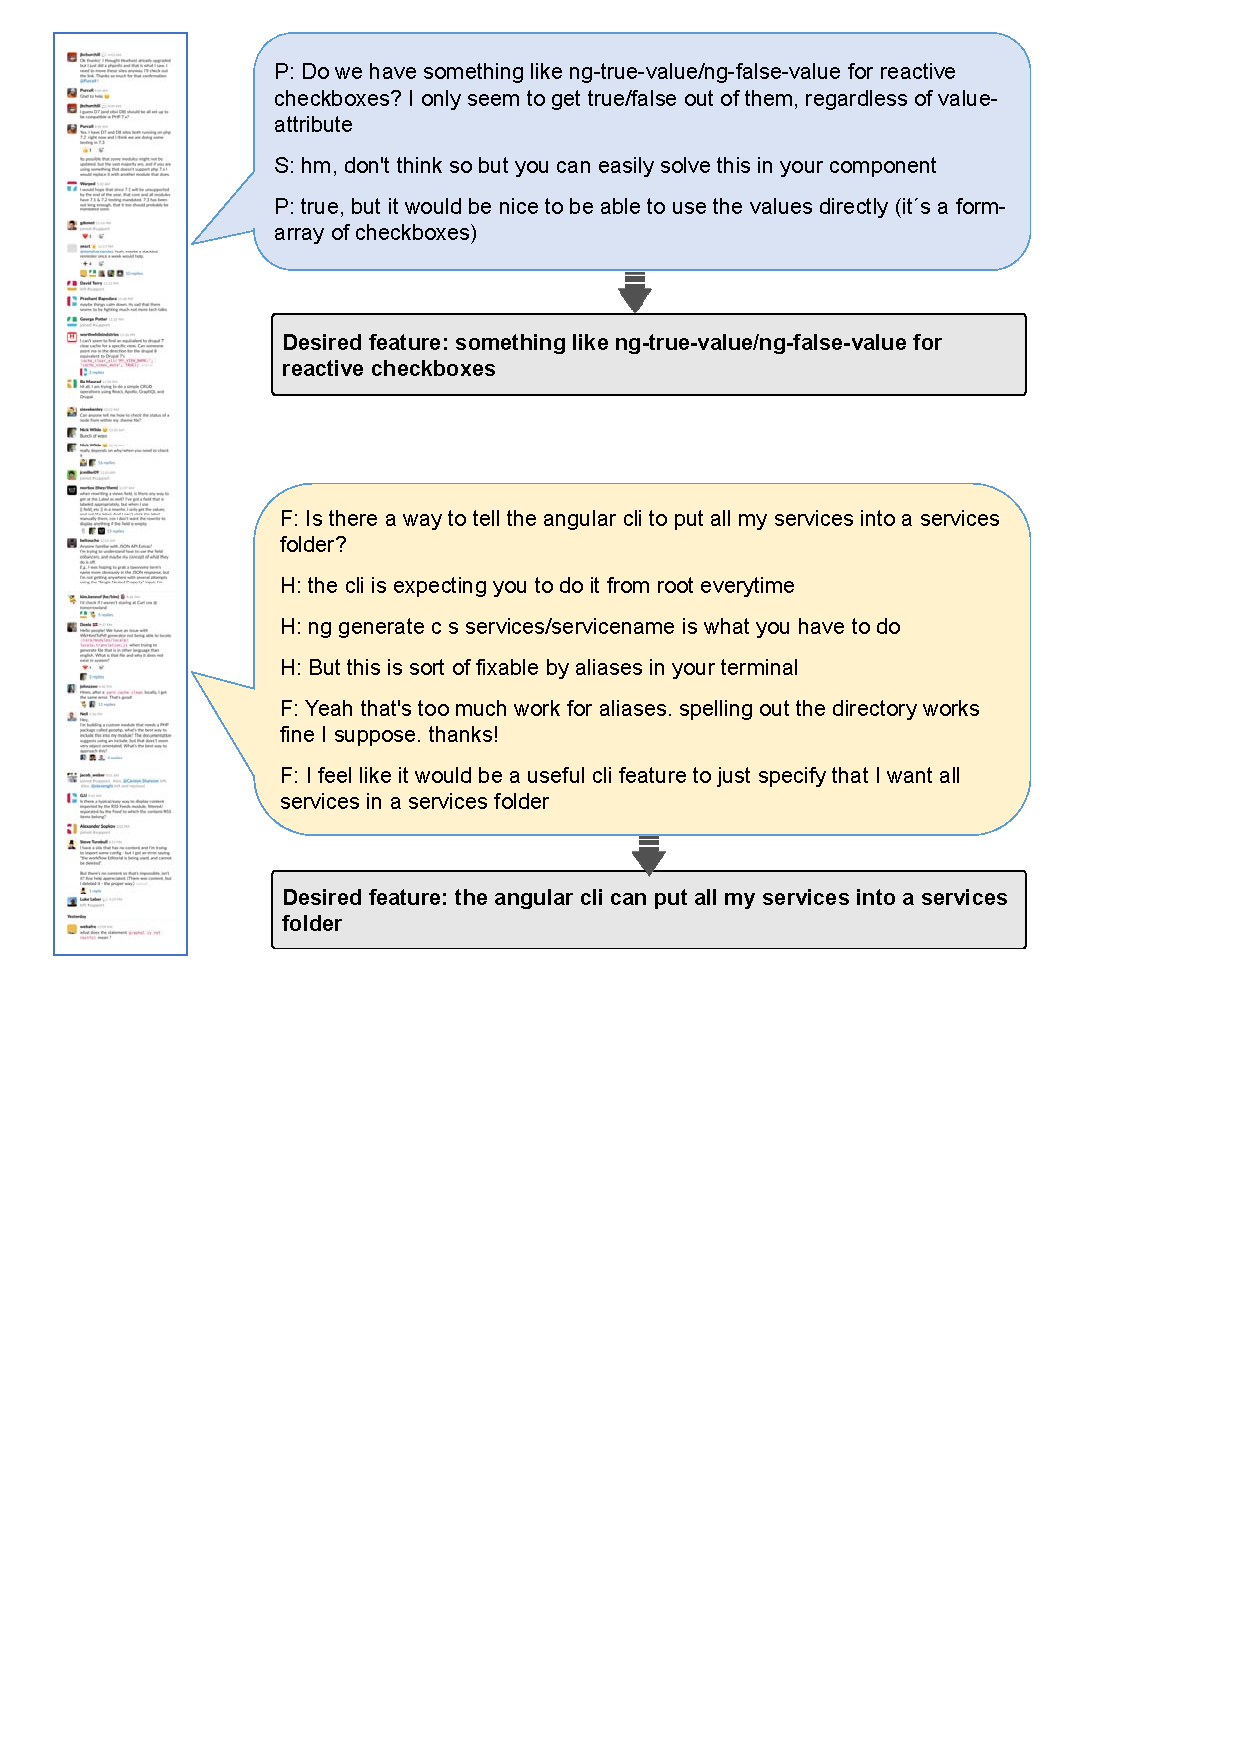
\includegraphics[width=0.70\textwidth]{Img/motivation.pdf}
    \bicaption{AngularJS项目的一个聊天信息例子,特征请求淹没在大量聊天历史中}{Example chat message from AngularJS project, where requests to desired features are buried in the massive chat history.}
    \label{fig:motivation}
\end{figure}

在这项工作中,我们将包含对新特征、增强特征的请求的对话视为特征请求对话。实际上,发布团队监视各种沟通渠道,以获取与下一个发布版本可能相关的多个信息源。如果发布团队可以从聊天消息中确认那些隐藏的特征请求,则他们的下一个发布计划可能会通过考虑实现更多特征请求而最大化利益相关者的满意度。

从大量的聊天消息中检索有价值信息的自动化挖掘技术需要从大量用户那里收集全面的特征请求,这有助于需求的确定和发布计划,进而促进软件开发的成功。尽管聊天消息数据源可能很庞大,并且随着时间的推移加入了了越来越丰富的特征请求,但是由于以下困难,要挖掘大量的聊天消息还是非常具有挑战性的。
\begin{enumerate}
    \item \textbf{对话层次分析:}分析来自聊天消息的对话不同于常规的句子级别的文本挖掘任务,因为它在理解一个句子时需要考虑对话范围内的上下文信息。因此,关于句子级别特征请求发现的现有研究不能直接用于此任务。例如,句子“我们需要添加垂直导航栏选项“被句子级别技术分类为特征请求。但是,当在在线聊天中发出时,后续对话指出现有功能可以以替代方式满足该请求。此外,句子级别的分类结果是不准确的,因为其在聊天消息中将大量离题句子识别为特征请求,例如,“我真的需要恢复我的编程技能“,”我想喝点咖啡和饼干“。
    \item \textbf{极其昂贵的标注:}聊天消息通常规模很大。在大量聊天消息之间查找特征请求对话,就像在大海捞针一样。由于庞大的语料库和少量正样本数据,标注聊天消息中的特征请求对话极其昂贵,只有少数聊天消息会被标注为特征请求类型。如何最大程度地利用少量标记数据来对未标记聊天消息进行准确分类成为一个关键问题。
    \item \textbf{耦合和噪声数据:}聊天消息通常是大规模的,并且是包含涉及广泛主题的非正式对话。两个或多个开发人员彼此同步地进行交互,其中他们的对话在聊天记录中很大程度上被耦合。此外,在聊天消息中存在噪声文本,例如重复消息和离题消息,这些消息不提供任何有价值的信息。耦合和噪声数据给分析和理解对话带来了困难。
\end{enumerate}

\section{研究内容和创新点}

因为用户和开发者之间、公司开发者团队内部之间等通常最先在开放式聊天平台显式或潜在地提出需求,里面会存在着大量的原始需求。聊天数据是需求的一个典型来源,一般会要求开发者在会话期间记录需求。并且聊天数据量一般较大,蕴含时间、用户角色等对需求十分重要的信息,我们可以从中挖掘出大量的用户的原始需求,并使用结构化的方式对其进行解释性说明,对通过传统方式发现需求的方式起到了启发、补充等作用。观察解耦后的会话可看出,对话中需求的表达形式因角色、上下文的不同而不同,有些显式地表达出清晰地需求,有些较为隐式地或者在交谈过程中逐步确定需求,因此,根据传统地基于规则地语义识别方法很难以及不能完整地识别并抽取需求,对此,我们使用深度学习基于对话形式进行需求识别和抽取。


本课题将主要从开放式聊天平台的数据出发,因聊天数据的规模较大、需求表述不规范、不明确、需求稀疏等问题,我们利用需求工程以及自然语言处理、机器学习等技术抽取出需求会话,并对其进行推荐,以达到从源头出发发现需求,快速及时发现需求,可以减少开发人员在聊天过程中对需求的记录,避免丢失重要的关于需求的信息,并对传统需求发现方式起到启发,补充的目的。

在这项工作中,我们是首先在对话级别上进行分析的,该技术旨在自动检测聊天消息中发布的隐藏特征请求。我们提出了一种名为{\tool}的新方法,该方法可以通过深层的孪生网络从聊天消息中识别特征请求对话。为了更好地理解对话级别的上下文信息,我们首先基于双向LSTM(BiLSTM)结构构建了一个上下文感知对话模型,该模型可以深入学习正向和反向对话的上下文信息。受到通过利用少量的标记资源来建立预测模型的少样本学习技术的启发,我们将把单个对话分类到其类别的传统文本分类任务转换为确定两个对话属于相同还是不同类的任务。因此,我们将上下文感知对话模型与孪生网络相结合,以学习一对对话之间的相似性,而不是单一对话类别的方式。特征请求对话的预测结果可以基于相似性预测及其配对对话中观察到的类别来推断。为了评估我们提出的方法,我们标注了三个流行的开源项目中的1,035个对话。实验结果表明,我们的方法明显优于两个句子级别特征请求分类模型和四个传统文本分类方法,其平均精度,召回率和F1值分别为88.52%,88.50%和88.51%。结果证实,我们的方法可以有效地检测聊天消息中的隐藏特征请求,从而可以自动方式从大量用户收集全面的需求。

本文主要贡献主要有以下几方面:
\begin{enumerate}
    \item  我们是第一个提出从大量聊天消息中识别隐藏特征请求的,这些特征请求可以帮助进行全面的需求收集。
    \item 我们引入了一种解决方案,该解决方案可以通过结合孪生网络来基于有限的标注数据有效地预测特征请求对话,从而大大减轻了对有监督数据进行标注的负担。
    \item 我们在三个活跃的开源项目中评估了我们的方法,并进行了实验比较,结果表明所提出的方法优于现有的研究和四个文本分类方法。
    \item 可公开访问的数据集和源代码\footnote{https://github.com/FRMiner/FRMiner},以促进我们的研究及其在其他情况下的重用。
\end{enumerate}



\section{论文组织结构}
本文内容共分为六章,各章节的具体内容概述如下: 

第 1 章 绪论 

本章目的在于阐述从大规模聊天记录中进行特征请求自动识别和抽取的研究背景及研究意义,并对本文的主要研究内容以及创新点进行归纳。通过论述特征请求对话自动抽取的研究背景
及意义论证特征请求对话自动化识别的可行性以及必要性。并针对从大规模聊天记录中进行需求对话识别过程中存在的三大问题,即对话层次分析、标注成本大和噪声数据多提出本文的基于孪生网络和分层上下文敏感对话模型的{\tool},并介绍了本文的贡献点。以及通过介绍本文的组织架构对全文内容进行总结。 

第 2 章 国内外相关研究现状

本章目的在于介绍近年来围绕着需求发现的工作,主要包括基于手工设计规则和基于统计机器学习的方法。接下来介绍聊天对话文本在软件工程中的应用以及自然语言文本中针对对话解耦的相关工作。针对对话,我们介绍了自然语言处理中常见的文本嵌入式表示方法和分类方法,并对于对话标注困难、标注数据量少的情况介绍了少样本学习。

第 3 章 需求对话识别模型结构设计

本章目的在于介绍我们提出的{\tool}模型结构和类别推断。首先介绍了朴素分层上下文敏感模型,然后利用孪生网络构建针对Pair-Instance的分类器,并且大大增强了数据量。最后,介绍了针对Pair-Instance进行目标对话的类别推断。

第 4 章 需求对话识别模型数据集构建和模型实现

本章目的在于介绍从数据集爬取、文本预处理、对话解耦、数据标注的数据集构建过程。然后,分别介绍分层上下文敏感对话模型和孪生网络的工程实现。接下来,介绍了模型训练过程和参数微调。最后,我们说明了{\tool}在工业场景部署的步骤。

第 5 章 需求对话识别模型验证与分析

本章目的在于介绍本文三个实验,即FRMiner的需求识别的有效性实验、孪生网络在FRMiner中的有效性实验、FRMiner的跨项目实验的实验设置。接下来针对实验结果进行分析,并论证了我们方法的有效性。

第 6 章 总结与展望

本章目的在于对全文内容进行总结,指出本文研究工作中可以进一步改进的地方,并介绍下一步工作进展计划。 


\section{本章小结}

本章通过论述本文的研究背景及意义证实基于大规模聊天记录进行需求对话识别和抽取的可行性以及必要性。并针对目前需求识别过程中存在的问题提出本文的研究内容以及创新点。最后,通过介绍本文的组织架构对全文内容进行总结。 
\chapter{国内外相关研究现状}\label{chap:related_work}

目前,国内外针对从非结构化文本中进行需求发现和提取已经有一些研究成果。
% 在许多开源和工业项目中,开发人员大量使用书面沟通渠道,例如邮件列表,issue tracker、聊天工具等,并且这样的方式已经遍布全球开发人员的日产工作中。
通过应用一些自然语言处理技术和文本挖掘如情感分析、话题建模、机器学习等技术,研究人员可以对这些非结构化文本进行意图分类,分类为如缺陷报告、解决方案、需求等类别\cite{maalej2015bug},其中识别到的需求可以服务于发布计划工具、向应用开发者提供支持,并决定哪些新功能需要在下个版本中实现。本章主要从需求对话识别工具构建过程中所涉及的相关概念以及技术细节,包括基于文本数据的需求发现、聊天对话文本在软件工程中的应用、文本分类以及少样本学习几方面进行探究并介绍国内外相关研究工作。

\section{基于文本数据的需求发现}


目前,人工和自动分析比如基于规则的方法以及有监督的机器学习方法正在被大量应用在分析对软件工程师和非专家的利益相关者有用的信息,如需求等信息中\cite{Morales2019Speech},并已有大量相关的研究工作。
\subsection{基于手工规则的需求发现}

RE Vlas等人\cite{morales2014discovering}提出一种基于语法的需求发现工具。作者使用Subject-Action-Object(SAO)语法标签对需求进行解析和表示。其中subject是需求声明的发出者,action定义了需求里面定义的特征,object表示被action影响的对象。比如:“这个提交按钮应该把表单数据提交给处理组件”中,“提交按钮”是subject,“发送”是action,object是“表单数据”。图\ref{fig:sao}是SAO方法对密码安全特征需求进行识别的一个例子。
\begin{figure}[htbp]
    \centering
    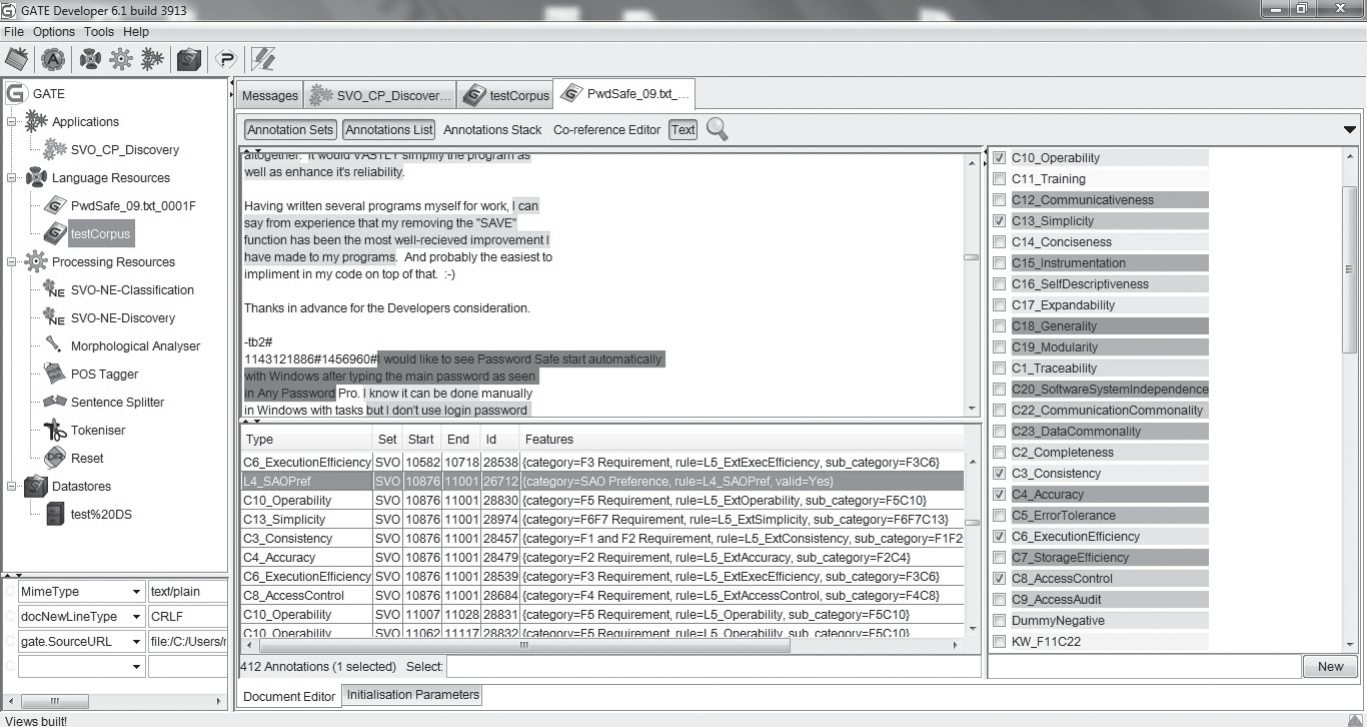
\includegraphics[width=0.70\textwidth]{Img/sao.png}
    \bicaption{基于SAO方法对密码安全特征需求进行识别}{SAO-based Recognized Password Safe Feature Requirements}
    \label{fig:sao}
\end{figure}


邮件是开发者之间进行沟通的重要方式之一,通常包含需求、观点询问、问题发现、解决方案、信息提供等不同类别的信息。Di Sorbo等人\cite{Sorbo2016Development}提出一种名叫DECA(开发者电子邮件内容分析器)的半监督学习方法,通过使用自然语言解析工具分析文本的语言学特征并且从询问帮助、提供帮助、提出新需求、报告或者讨论BUG等几方面对开发者的意图进行分类。Di Sorbo等人首先根据来自Ubuntu和QT的数据设置更适合邮件列表信息的分类,具体分类类别如表\ref{tab:deca0}所示。
\begin{table}[htb]
\bicaption{句子例子以及对应的类别}{Sentence examples and corresponding categories}
    \label{tab:deca0}
    \centering
    \footnotesize% fontsize
    \setlength{\tabcolsep}{4pt}% column separation
    \renewcommand{\arraystretch}{1.2}%row space 
\begin{tabular}{lcccccccc}
\hline
句子类别的例子      & 分类类别 \\
\hline
讨论一个变更       & 需求 \\
定位BUG        & 问题发现 \\
BUG是否被修复     & 信息询问 \\
针对已知问题提出解决方案 & 解决方案 \\
请求其他开发者做出变更  & 需求 \\
询问代码时如何工作的   & 信息询问 \\
询问为何这样写代码    & 信息询问 \\
向某人征求意见      & 意见询问 \\
找出代码作者       & 信息询问 \\
更多的了解代码      & 信息询问 \\
告诉其他开发者一些事情  & 信息提供 \\
\hline
\end{tabular}
\end{table}
然后对其进行手工标注,作者发现开发人员在关于开发问题的讨论中撰写关于现有错误或者建议提出需求时,他们倾向于使用一些经常性的语言模式,比如对于“我们可以使用漏桶算法来限制带宽”,可以发现句子中提供一个明确定义的谓词-参数结构,对此,可以看出大多数具有谓词-论元结构的句子表明解决方案。作者定义了启发式规则,首先发现句子的特定句法结构,然后推广某些类型的信息,最后忽略无用的信息。所以,作者定义了“【某人】可以使用【某事物】”的一般模式来识别解决方案。图\ref{fig:deca1}是作者通过斯坦福依存句法分析来分析启发式规则时的例子。
\begin{figure}[htb]
    \centering
    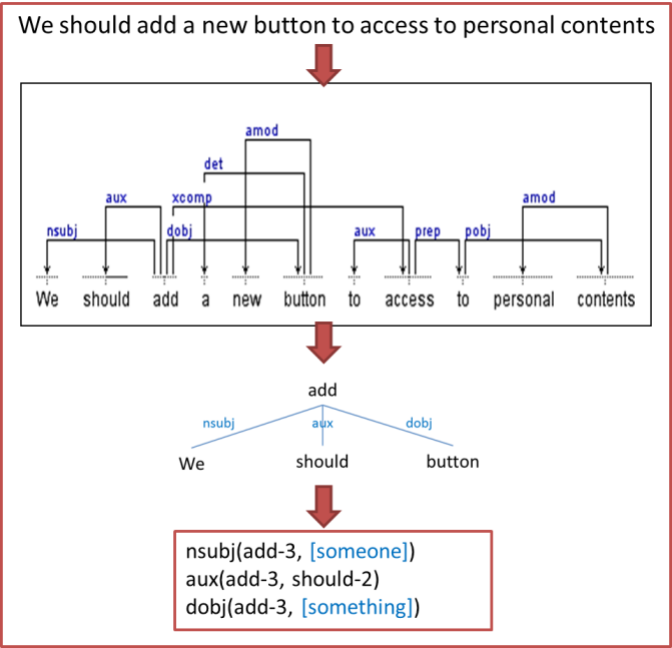
\includegraphics[width=0.60\textwidth]{deca1}
    \bicaption{需求文本中的自然语言解析树}{Natural language parsing tree about feature request}
    \label{fig:deca1}
\end{figure}
作者通过图\ref{fig:deca1}定义了“【某人】应添加【某事物】”的启发规则并于需求相关联。Andrea Di Sorbo等人的观点是在软件工程领域存在相关的重复语言模式,这对软件过程中的需求分析非常有用。

L Shi等人\cite{shi2017understanding}提出利用自然语言处理技术生成一组模糊规则来自动分析需求的方法,其将需求中的每个句子进行分类,类别有意图、解释、益处、缺点、示例和无关,分类的结果用来增量生成模糊规则。作者定义了这些类别以及类别的定义和优先级来帮助结构化表示需求,并重点显示值得关注的内容,如表\ref{tab:fra0}所示。
\begin{table}[htb]
\bicaption{句子类别的定义}{Definitions of sentence categories}
    \label{tab:fra0}
    \centering
    \footnotesize% fontsize
    \setlength{\tabcolsep}{4pt}% column separation
    \renewcommand{\arraystretch}{1.2}%row space 
\begin{tabular}{lcccccccc}
\hline
类别 & 重要性 & 定义                     \\
\hline
意图 & 1   & 关于改进系统和功能的主意、需求、期望的描述  \\
益处 & 2   & 关于提出的需求带来的好处和有帮助的结果的描述 \\
缺点 & 3   & 关于当前系统行为的缺点            \\
例子 & 4   & 关于支持提出的需求的例子           \\
解释 & 5   & 关于提出需求的场景和解决           \\
无关 & 6   & 和系统无关的信息              \\
\hline
\end{tabular}
\end{table}
作者分别在词汇、语法、语义三个级别启发式地定义模糊规则。词汇通过设置不同类别句子的词汇表来对句子进行分类,句法通过对句子进行依存结构分析不同句子类别的句法特征,语义层面通过定义在某个类别的句子中的语言表达的含义,如图\ref{fig:fra1}所示的语义模式。
\begin{figure}[htb]
    \centering
    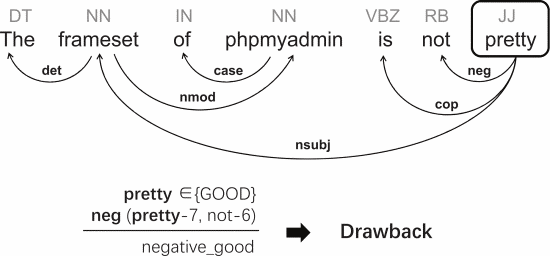
\includegraphics[width=0.70\textwidth]{fra1}
    \bicaption{缺陷类别的语义模式示例}{An example about semantic pattern of defect class}
    \label{fig:fra1}
\end{figure}
实验表明,随着新规则的引入,模糊规则的分类性能越来越高。此外,在将模糊规则转换成布尔变量之后,将其应用于各种机器学习算法上得到了更好的效果。

I Morales-Ramirez等人\cite{Morales2019Speech}关注于分析在线讨论,如开源软件的邮件列表和用户论坛,在这里,不同的利益相关者比如开发者、软件终端用户会讨论有助于软件发展的信息。基于规则Speech-acts分析\cite{morales2014discovering}用在线讨论的自动分析上,比如可以通过学生的查询理解学生的意图\cite{feng2006intelligent}等。 Speech-acts理论认为当某人说一些话存在一些模式让对方相信或者做出对应的行为\cite{acts1969essay},比如在询问一个新功能中使用的词汇模式包括:“添加特征”、“想要这个特征”等。作者把不同speech-acts规则归为几类:c-Assertive, c-Responsive, c-Requestive和c-Attachment。如表\ref{tab:speech-act0}所示,每一列为对应的独立speech-acts类别。
\begin{table}[htb]
\bicaption{Speech-acts列表}{List of speech-acts}
    \label{tab:speech-act0}
    \centering
    \footnotesize% fontsize
    \setlength{\tabcolsep}{4pt}% column separation
    \renewcommand{\arraystretch}{1.2}%row space 
\begin{tabular}{lcccccccc}
\hline
c-Assertive & c-Requestive & c-Responsive & c-Attachment & c-Other          \\
\hline
断定        & 请求         & 回应         & 附件         & 描述性的      \\
确认        & 需求         & 建议         & 代码         & 接受           \\
让步        & 问题         & 支持         & URL链接      & 拒绝           \\
            &              &              & 日志文件     & 消极观点 \\
            &              &              &              & 积极观点  \\
            &              &              &              & 感谢            \\
            &              &              &              & 内容丰富的 \\
\hline            
\end{tabular}
\end{table}
基于Speech-acts的模型结构如图\ref{fig:speech-acts1}所示。
\begin{figure}[htb]
    \centering
    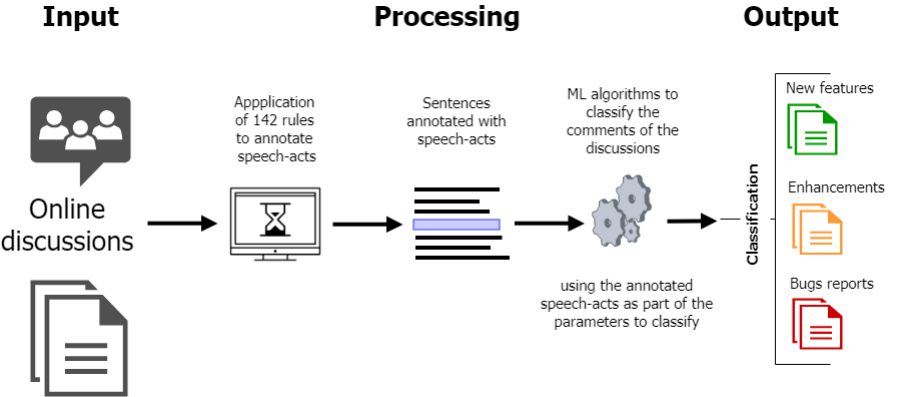
\includegraphics[width=0.70\textwidth]{Img/speech-acts1.png}
    \bicaption{基于Speech-acts的分析模型}{Speech-acts based analysis approach}
    \label{fig:speech-acts1}
\end{figure}
这个工具结合了作者关于需求的知识,以及利益相关者在在线讨论中表达需求的方式来定义142条词法-句法规则,从而对需求进行识别。

\subsection{基于统计机器学习的需求发现}
开发者和客户通常会通过会议来获取用户故事,P Rodeghero等人\cite{Rodeghero2017Detecting}提出一种从客户和开发人员之间记录的对话中自动提取和用户故事相关信息的方法。作者从对话记录中自动提取用于构建用户故事的数据,分别进行定性研究,其可以检验对话中包含用户故事的角色、功能和基本原理的假设;以及定量研究以确定现有分类算法的效果。通过定性研究分析得到大约5.5\%的对话包含功能信息,2.9\%包含了基本原理,只有0.5\%讨论了角色,发现对话包含重要的功能和基本原理信息,但关于角色的数据非常有限。作者训练了一个分类器用于检测包含功能数据的对话部分。在数据收集部分,作者收集一家软件开发公司的会议记录,并标注文件名、会话、摘要、会话转折、角色、功能、理由等信息,对会议记录提取了25个属性进行分类,分析的单位是转折而不是句子,提出的方法模型如图\ref{fig:Rodeghero2017Detecting}所示。
\begin{figure}[htb]
    \centering
    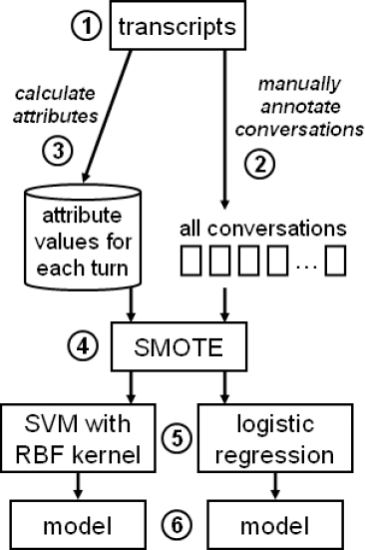
\includegraphics[width=0.40\textwidth]{Rodeghero2017Detecting.png}
    \bicaption{分类器模型结构图}{Structure of classifier}
    \label{fig:Rodeghero2017Detecting}
\end{figure}

Q Huang等人\cite{Huang2018Automating}发现Di Sorbo等人的分类类别还有55\%的句子不能覆盖,于是在其分类的基础上合并了两种意图,并新增了两种意图,提炼过的分类类别如表\ref{tab:aim0}所示。
\begin{table}[htb]
\bicaption{精炼后的意图分类}{Intention classification after refine}
    \label{tab:aim0}
    \centering
    \footnotesize% fontsize
    \setlength{\tabcolsep}{4pt}% column separation
    \renewcommand{\arraystretch}{1.2}%row space 
\begin{tabular}{lcccccccc}
\hline
类别   & 描述                 \\
\hline
信息提供 & 将知识、经验、计划、更新共享给其他人 \\
信息寻找 & 希望得到信息和帮助          \\
需求 & 帮助改进现有功能或提出新功能     \\
解决方案 & 共享可能的解决方案          \\
问题发现 & 报告BUG,或描述异常行为      \\
侧面评价 & 表达观点或进行评价          \\
无意义  & 无意义的或不重要的         \\
\hline
\end{tabular}
\end{table}
并提出了使用Convolutional Neural Network(CNN)\cite{kim2014convolutional}的方法自动将句子分类为不同的意图类别,整体模型架构如图\ref{fig:aim1}所示。
\begin{figure}[htbp]
    \centering
    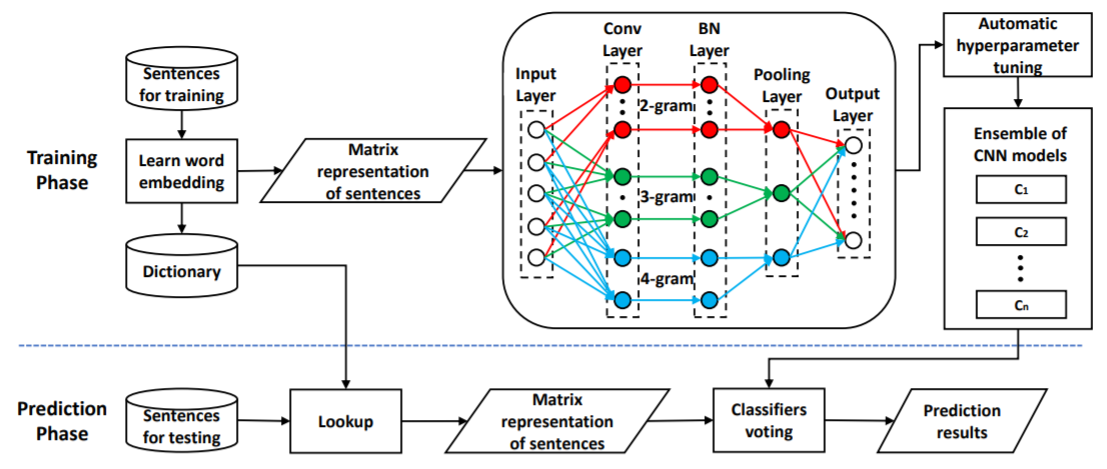
\includegraphics[width=0.8\textwidth]{aim1.png}
    \bicaption{CNN分类模型整体框架}{Structure of CNN classifier}
    \label{fig:aim1}
\end{figure}
CNN将句子作为输入,输出7个概率值,从而得出概率最大的句子类别,即使测试集中没有出现和训练集相似的模式或者关键词,模型也会给出概率最大的类别,从而覆盖所有句子。

% Y Zhang等人\cite{zhang2015sensitivity}发现词向量的维度、过滤器的数量以及过滤器的深度是对效果影响较大的超参数,作者使用贪婪的方式搜索最优参数。
D Arya等人\cite{arya2019analysis}通过对15个问题讨论进行内容定量分析,确定了包括潜在需求在内的16种信息类型。作者手工构建了14个对话特征,并使用随机森林作为分类器,对表达新需求的句子可以达到66\%的F1值。
W Maalej等人\cite{maalej2015bug}使用自然语言处理技术包括文本分类、情感分析把App Reviews分类为缺陷报告、需求、用户经验和打分。其中分类结果的precision可达到70-95\%,recall可达到80-90\%。

\section{聊天对话文本在软件工程中的应用}
在各种软件开发项目中,两种常见的聊天方式为同步和异步沟通方式\cite{yu2011communications}。同步方式包括Internet Relay Chat(IRC)等聊天工具,异步方式包括邮件列表、issue tracker等工具。
% 目前已有大量的研究工作正在开发有效的工具支持软件分析,它们利用自然语言处理技术从应用商店评论、在线聊天记录、邮件列表、用户论坛等文本数据中抽取相关信息,并且使用文本挖掘和机器学习技术对信息进行分类如缺陷报告或者需求。
其中基于Web平台的关于软件应用和服务的在线聊天讨论中包含着关于软件系统的丰富的信息,并在包括需求发现等各种软件工程任务中表现出来巨大的价值\cite{Morales2019Speech}。

B Lin等人\cite{lin2016developers}通过一项关于开发者怎么使用Slack、哪个聊天工具在开源社区比较流行、聊天工具能够为软件开发带来怎么样的好处的研究,发现开发者使用Slack进行个人、团队、社区级别的交流,Slack也占据越来越重要的地位,在某些情况下会代替邮件。
E Shihab等人\cite{shihab2009studying}通过两个大型开源项目从几个维度分析了开发者IRC会议:会议内容、会议参与者、他们的贡献、会议类型。作者的研究表明IRC正在开源社区占据越来越重要的地位,强调了从开发者聊天记录中可以获取丰富的信息。
P Chatterjee等人\cite{chatterjee2019exploratory}调查了通过挖掘开发者谈话从而支持软件维护和演化的有效性和挑战性,作者发现开发者倾向于通过即时聊天工具分享对于观点或者有意义的想法,并且说明了通过应用一些技术和训练集可以达到较高的对话解耦效果。



\section{文本分类方法}
\subsection{朴素贝叶斯}
朴素贝叶斯(Naive Bayesian)\cite{mccallum1998comparison}是基于词袋假设和贝叶斯公式的常用文本分类模型。对于文档$d$和类别$c$,该文档属于类别$c$的概率为$P(c|d)=\frac{P(d|c)P(c)}{P(d)}$,其极大后验也即最有可能的类别为$c_{MAP}=\mathop{\arg\max}\limits_{c \in C}P(c|d)$,去掉贝叶斯公式分母可得$c_{MAP}=\mathop{\arg\max}\limits_{c \in C}P(d|c)P(c)$,基于词袋模型和特征条件独立性假设可得
$$c_{NB}=\mathop{\arg\max}\limits_{c \in C}P(x_1|c)P(x_2|c)\dots P(x_n|c)P(c)=\mathop{\arg\max}\limits_{c \in C}p(c)\prod\limits_{x \in X}P(x|c)$$
因此,通过极大似然估计获得似然概率$P(x|c)$和先验概率$P(c)$即可得到后验概率$P(c|d)$,然后将后验最大的类别作为分类结果。

\subsection{fastText}
fastText\cite{joulin2016bag}是Facebook开源的一个词向量计算和文本分类工具。
% ,其优点主要在于在文本分类任务中,fastText(浅层网络)往往能取得和深度网络相媲美的精度,却在训练时间上比深度网络快许多数量级。在标准的多核CPU上,能够在10分钟之内训练10亿词级别语料库的词向量,在1分钟之内能够分类有30多万类别的50多万条句子。
其模型架构和word2vec\cite{mikolov2013distributed}的CBOW模型架构非常相似,图\ref{fig:fasttext}所示为fastText的模型结构图。
\begin{figure}[htb]
    \centering
    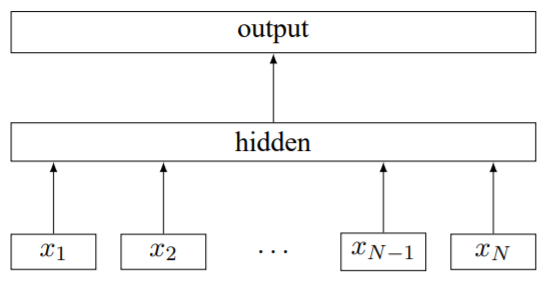
\includegraphics[width=0.6\textwidth]{Img/fastText.png}
    \bicaption{对于具有N ngram句子特征$x_1, \dots , x_N$ 的句子的fastText模型结构。特征被嵌入表示并且求平均来作为隐藏特征}{Model architecture of fastText for a sentence with N ngram features $x_1, \dots , x_N$ . The features are embedded and averaged to form the hidden variable}
    \label{fig:fasttext}
\end{figure}
fastText模型结构类似于CBOW只有三层,并且也利用了分层的Softmax减少训练时间。但是CBOW的输入是目标单词的上下文窗口,fastText的输入是用来表示单个文档的多个单词及其n-gram特征。CBOW的输出是目标词汇,fastText的输出是文档对应的类别。并且fastText将单词的字符级别的n-gram向量作为输入的额外特征。

\subsection{随机森林}
随机森林(Random Forest)\cite{liaw2002classification}
随机森林是一种集成机器学习中Bagging的方法,其是由很多决策树构成的,不同决策树之间是独立的。如图\ref{fig:rf-model}所示,当进行分类任务时,对于新的输入样本,森林中的每一棵决策树对其分别进行判断和分类,每个决策树会得到一个自己的分类结果,决策树的分类结果中哪一个分类最多,那么随机森林就会把这个结果当做最终的结果。
\begin{figure}[htb]
    \centering
    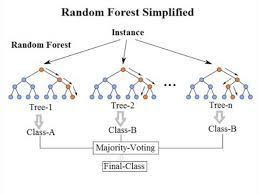
\includegraphics[width=0.6\textwidth]{Img/rf-model.jpg}
    \bicaption{随机森林模型架构}{Model architecture of Random Forest}
    \label{fig:rf-model}
\end{figure}
它的构造过程首先对数据集合进行有放回的抽取,得到若干个子数据集,对于每个数据集中随机选取的特征,使用信息增益进行分裂,然后得到若干树组成森林。由于随机森林选取数据集和特征的随机性,其优点在于不容易过拟合,处理很高维度的数据,并且不用做特征选择,由于决策树并行生成,因此可以并行训练。

\subsection{梯度提升决策树}
梯度提升决策树(Gradient Boosting Decision Tree)\cite{ke2017lightgbm}
梯度提升树是另一种基于树的集成机器学习方法,其模型定义为加法模型:
$$f_M(x)=\sum^M_{m=1}\alpha_mh_m(x,\theta_m)=\sum^M_{m=1}f(x,\theta_m)$$,其中$h_m$是第m棵树,$\alpha_m$是第m棵树的权重。GBDT目标函数为:
$$\large {r_{mi}} = -\left[\frac{\partial L(y_i,f(x_i))}{\partial f(x_i)} \right]_{f(x)=f_{m-1}(x)}$$,使用平法误差损失函数时$L(y, f(x)) = (y-f(x))^2$。其使用经验风险最小化求得下棵树的参数:
$$\hat \theta_{m} = \mathop{\arg\min}\limits_{\theta_{m}} \sum_{i=1}^ML(y_{i}, f_{m-1}(x_{i})+T(x_{i}; \theta_{m}))$$

\section{少样本学习}
深度学习在计算机视觉和NLP领域都取得了巨大的成功。但是它严重依赖于足够多的训练数据量,并且当标记的资源不足时,很难达到很好的效果。

基于在线聊天消息的自动挖掘技术面临标注资源不足的问题,在在线聊天中,开发人员会在短时间内创建大量的讨论对话。为了学习有效的模型,需要从这些大量讨论文本中标注对话数据,这是一项非常耗时的工作,因为这些对话数据不仅文本很长、掺杂大量无关信息,而且标注人员还需要有领域知识来对对话进行充分的理解。

对此类标注数据困难的情况,少样本学习被提出来克服这些问题\cite{wang2019few},其旨在通过学习少量样本以及对应的标签信息从而对提高对新样本的学习能力。少样本学习可以分为以下三类\cite{chen2019closer}:基于模型的方法:其旨在通过模型设计出发,从少量标注数据的分类任务中学习映射函数;基于优化的方法:其可调整传统的梯度下降优化器方法以拟合数据分布;基于度量的方法:其通过学习相似性度量函数对样本进行分类。

\subsection{基于模型的少样本学习方法}
A Santoro等人\cite{santoro2016one}提出的使用记忆增强的方法来解决少样本问题是基于模型方法的一个代表。由于神经网络图灵机(NTMs)能通过外部存储(external memory)进行短时记忆,并能通过缓慢参数更新来进行长时记忆,文章使用NTM来存储样本以及对应类别表示信息,当需要预测一个已经模型已经见过的样本时,这些信息可以相应的被检索,因此,文章方法可以快速准确地预测那些只出现过一次的数据。另一方面,如图\ref{fig:few-memory}所示,文章模型基于RNN结构,
\begin{figure}[htb]
    \centering
    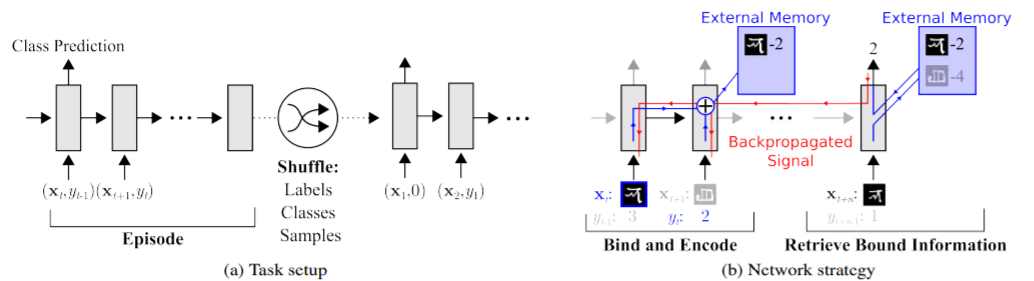
\includegraphics[width=0.8\textwidth]{Img/few-memory.png}
    \bicaption{基于外部知识模块的少样本学习方法}{The approach of few-shot learning based on external memory module}
    \label{fig:few-memory}
\end{figure}
模型将数据看成序列来进行训练,训练过程中将样本和标签对应,并更新外部知识模块,在测试时输入新的类的样本进行分类时,模型可以把未出现过的数据连接到对应相关的外部记忆模块中的表示,借助外部知识信息达到更好的分类效果。

\subsection{基于优化的少样本学习方法}
C Finn等人\cite{finn2017model}提出了一种模型无关的元学习方法,其可以快速拟合多种不同的包括分类、回归和强化学习等任务。文章的方法可以在小量样本上,用少量的梯度更新步骤来训练模型的初始化参数,从而可以获得较好的泛化性能,并且容易对模型进行微调。具体的,如图\ref{fig:few-optim}所示,该方法能够找对任务的损失函数敏感的参数$\theta$,
\begin{figure}[htb]
    \centering
    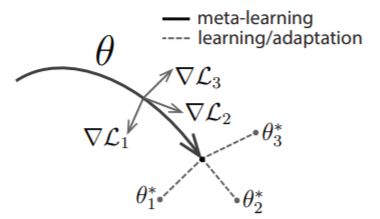
\includegraphics[width=0.6\textwidth]{Img/few-optim.png}
    \bicaption{模型无关的元学习算法}{The algorithm of Model-Agnostic Meta-Learning}
    \label{fig:few-optim}
\end{figure}
对参数$\theta$进行微小改变便能较大程度改善模型的损失函数、适应于不同任务并提高任务效果。



\subsection{基于度量的少样本学习方法}
孪生网络\cite{bromley1994signature}是一种基于度量的少样本学习技术,该技术被广泛用于衡量文本或图像之间的语义相似性\cite{mueller2016siamese}。传统的分类模型尝试学习从单个实例映射到其类别的函数空间,但是当可用的标注资源数据较少时,这些分类模型不能达到理想的效果。与传统方法不同,孪生网络将成对的实例作为输入,旨在学习来决定两个实例是否属于同一类别的关键特征。如图\ref{fig:siamese-model}所示,它由两个相同的子模块组成,这些子模块不仅共享模型结构,而且还共享参数。
\begin{figure}[htb]
    \centering
    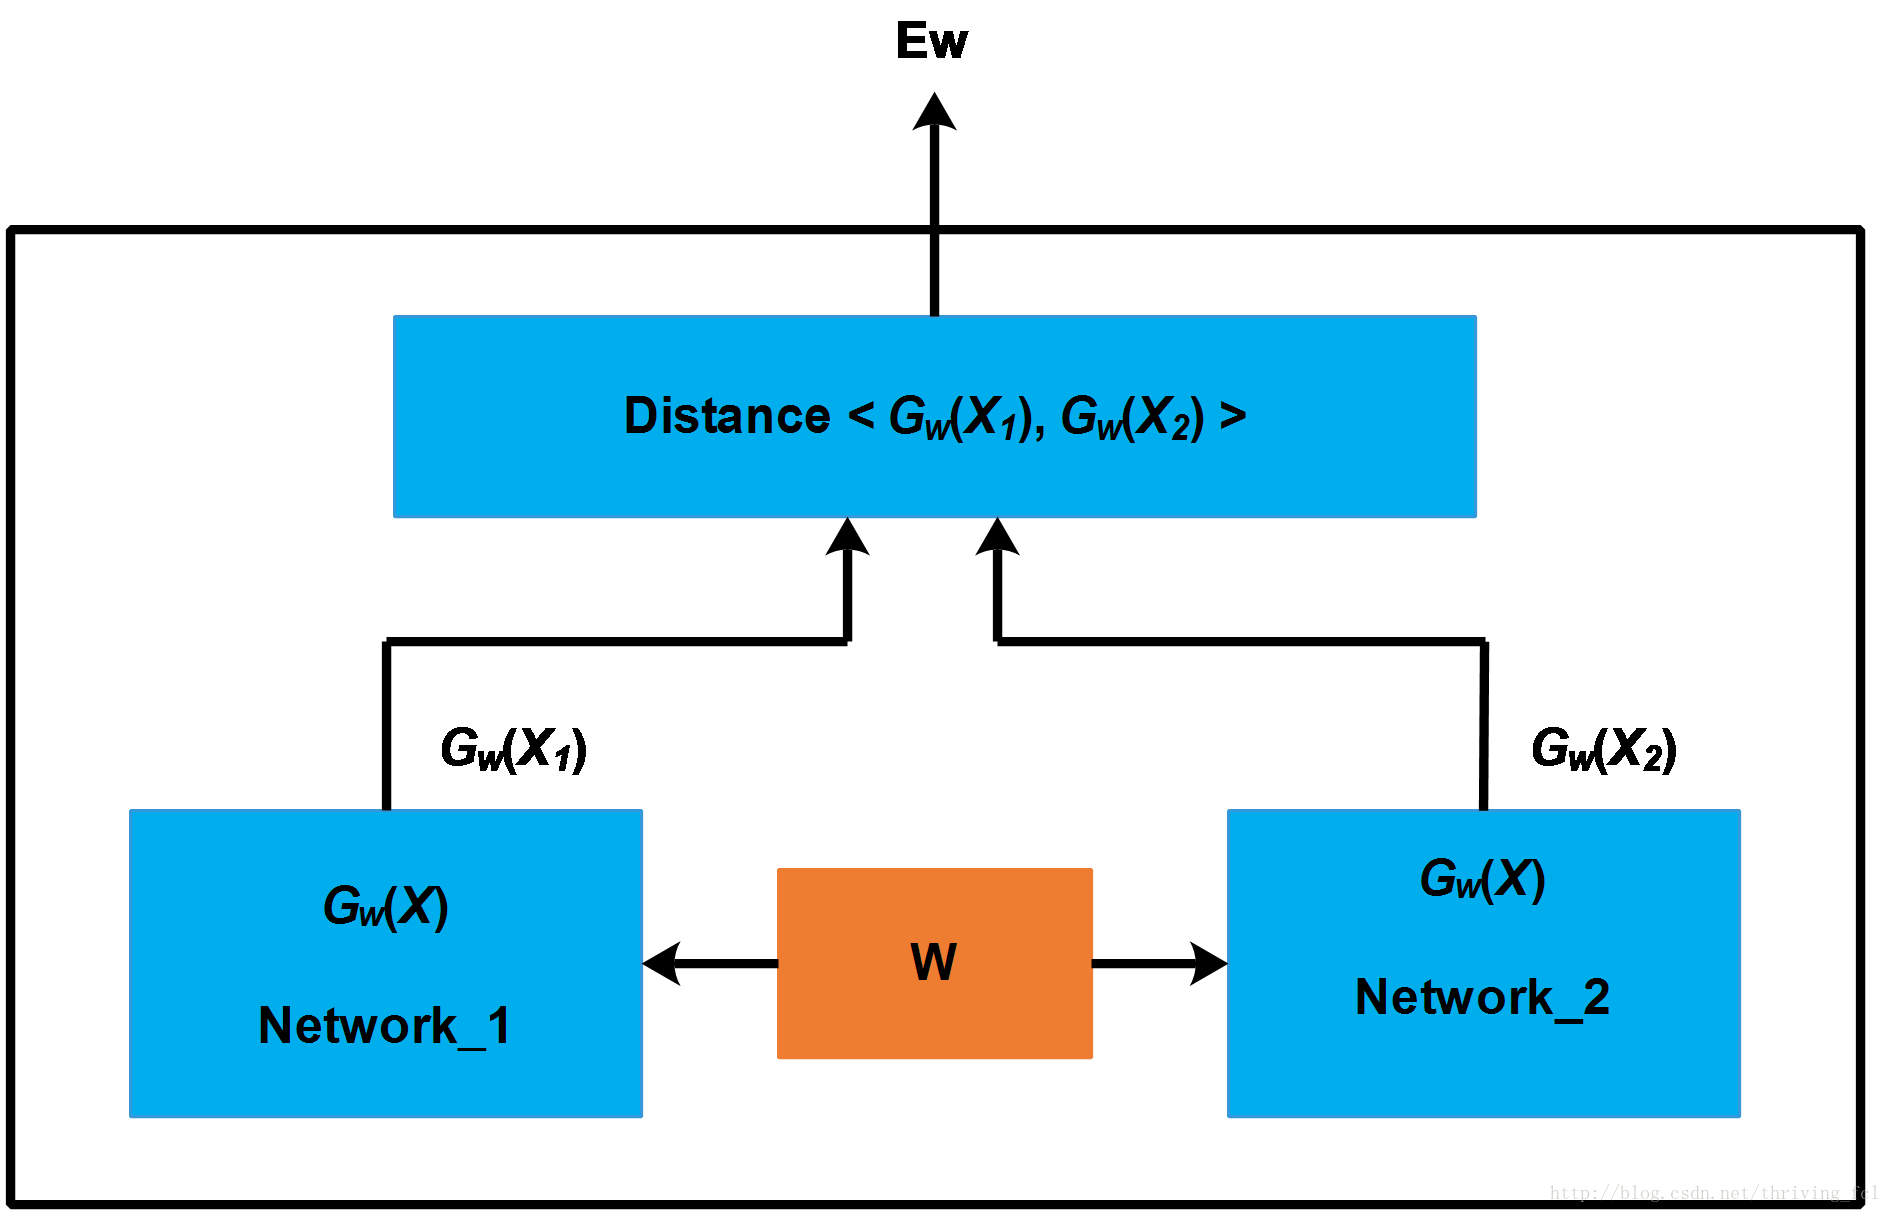
\includegraphics[width=0.6\textwidth]{Img/siamese-model.png}
    \bicaption{孪生网络模型架构}{Model architecture of Siamese Network}
    \label{fig:siamese-model}
\end{figure}
其中,Network\_1和Network\_2分别接收两个输入$X_1$与$X_2$,将其转换为向量$G_w(X_1)$与$G_w(X_2)$,再通过某种距离度量的方式计算两个输出向量的距离$E_w$。

本文由于以下原因采用孪生网络来解决样本数量的局限性。从直觉上讲,对于本任务而言,确定两个对话是否相似,要比为每个对话指定确切的类别更容易。另外,由于孪生网络将一对对话作为输入,因此数据集从元素级别转换为成对级别,可以通过对话之间的排列组合进行数据增强。

\section{本章小结}

本章主要针对在构建本文提出的基于孪生网络从大规模聊天记录中进行隐藏需求对话识别的方法时涉及到的相关概念和关键技术进行详细调研和总结。其中基于文本数据的需求发现主要包括基于手工设计规则和基于统计机器学习的方法,它们在不同的数据来源包括issue tracker、邮件列表等取得了较好的效果;聊天对话文本目前被广泛运用在软件工程中,并被当作丰富的信息来源;对于对话文本分类,本章介绍了常见的、效果稳定的文本分类模型;针对对话数据标注困难、样本少的情况,介绍了当前常见的包括孪生网络等的少样本学习技术。


\chapter{上下文敏感对话模型}
本章节介绍本文设计的使用TextCNN和BiLSTM构建分层的上下文敏感对话模型{\dm},旨在分别从句子级别和对话级别对对话文本进行语义表示。首先,通过对聊天消息进行解耦来获取独立解耦对话,然后以对话作为输入文本构建一个分层的上下文敏感对话模型,上下文敏感对话模型{\dm}使用基于TextCNN\cite{kim2014convolutional}对句子进行向量化表示,接下来这些句子向量作为输入,并以对话中对应序列通过BiLSTM\cite{graves2013speech}结构进行编码并获得对话的语义表示。


\section{聊天信息中的对话解耦}
在线聊天是开发者社区之间的一种同步文本通信方式,当一组人在公共的聊天平台进行通信时,聊天中的消息形成流式信息,往往会有很多的对话同时出现,并且经常出现耦合的情况,例如单个会话会与其他会话交织在一起。并且如同 Internet Relay Chat(IRC)、Google Hangout、网站评论等聊天平台不能显式地表明对话的结构,所以无法从中获取独立的会话信息。

将聊天消息划分为一组不同的对话是任何上层对话分析的基本前提,对话解耦就是从一个单一的流信息中识别独立对话的一个任务。
% 目前,关于对话解耦做出重要贡献的是一系列在IRC上标注的数据和训练的模型。Adams和 Martell等人\cite{adams2008topic}研究了对话解耦和话题识别,但是没有公开数据集。Riou等人\cite{riou2015using}在IRC的\#Ubuntu-fr Channel标注对话以及句子关系。Lowe等人\cite{lasecki2013conversations}启发式地从\#Ubuntu Channel进行对话抽取。他们的工作提供了930,000个解耦的对话,为其他对话解耦工作提供了数据基础。Elsner和Charniak等人\cite{elsner2008you}探索了使用信息对特征集和线性分类器,结合局部和全局的推断方法。Jiang等人\cite{jiang2018learning}使用了神经网络的方法,效果达到了提升。
JK Kummerfeld等人\cite{kummerfeld2018large}手工标注了一个大小为77,563条的解耦对话,对于对话定义了一个回复关系图模型,数据集包含内部的对话结构。如图\ref{fig:example-conversation}所示的两个耦合的对话和一个标注的图结构数据是标注数据集的一个样例,其中不同颜色的连线表示图连接。这个例子包括一个当多个人独立的尝试帮助BurgerMann时收到的多个回应的信息,并且在最后消息中BurgerMann回复多个信息。另外,也可以看到delire和Seveas两个用户同时参与两个交谈中。
\begin{figure}[htb]
    \centering
    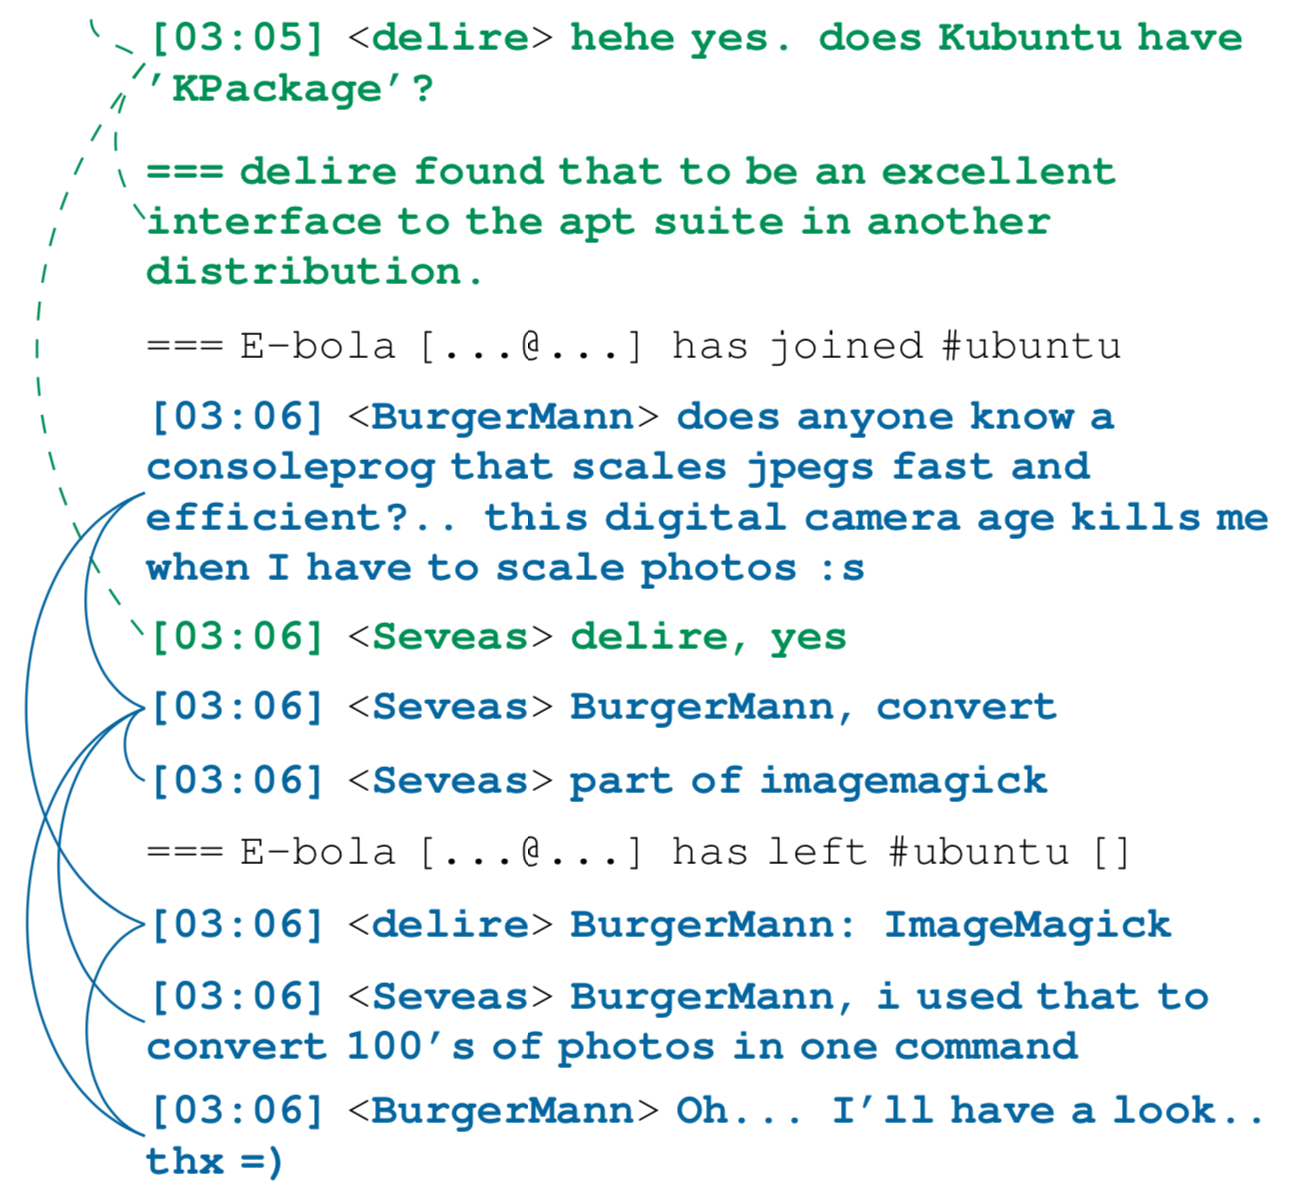
\includegraphics[width=0.4\textwidth]{Img/example-conversation.png}
    \bicaption{Ubuntu的例子。曲线是回复图结构的标注,其中蓝实线和绿虚线分别代表两个对话}{\#Ubuntu log sample. Curved lines are graph annotations of reply structure, which define two conversations shown with blue solid edges and green dashed edges}
    \label{fig:example-conversation}
\end{figure}
作者设计了一个具有2层、512维隐藏层和sigmod非线性激活函数的浅层前馈神经网络,并手工设计了77个特征,其中每个元素都是从原始对话文本中提取的数字类别特征,其中包括当前用户发布的先前聊天消息的时间间隔、聊天内容中是否有目标用户、两个聊天文本是否包含相同的单词等。该模型可以达到74.9%的精度和79.7%的召回率,具有相对较好的效果。

由于JK Kummerfeld等人提出的对话解耦模型为当前效果最好的对话解耦模型,本文选用其研究工作中的模型结构和标注数据对原对话文本进行会话解耦。

\section{上下文敏感对话模型结构设计}
本文设计了一个分层的上下文敏感对话模型{\dm},该模型可以捕获对话中每个句子的语义以及对话整体上下文信息。如图\ref{fig:model}所示,上下文敏感对话模型由四层组成:输入层,句子表示层,对话表示层和输出层。
\begin{figure}[htbp]
    \centering
    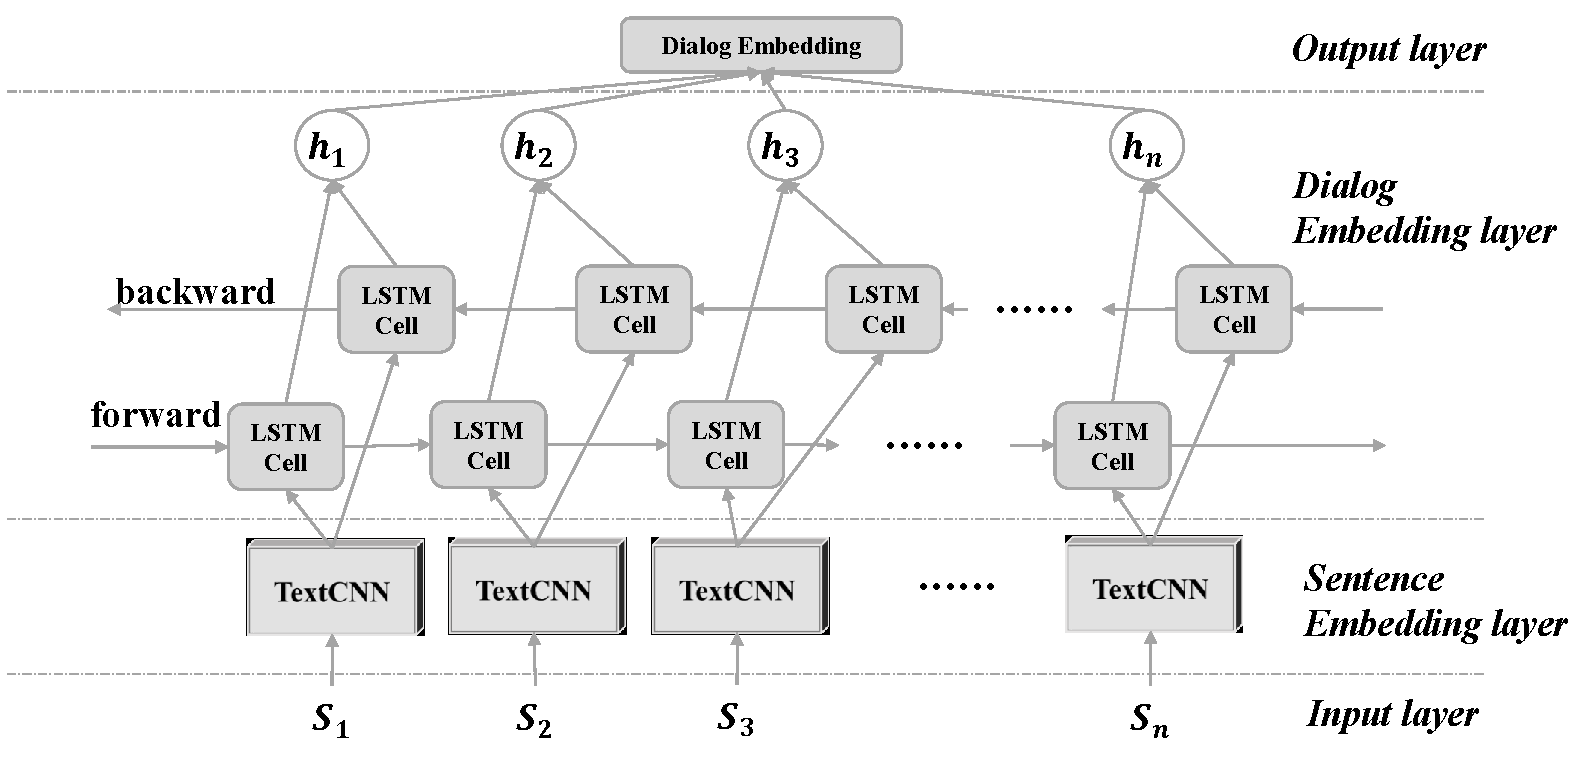
\includegraphics[width=\textwidth]{Img/dialog-model.pdf}
    \bicaption{分层的上下文敏感对话模型{\dm}}{Hierarchical Context-aware Dialog Model {\dm}}
    \label{fig:model}
\end{figure}


% \subsection{BiLSTM}


\subsection{输入层设计}
本文首先将句子分词作为基本元素,然后将词转换为对应的词向量作为模型输入。为了获得更好的效果,本文利用预先在Wikipedia和Gigword语料库上的60亿个单词上经过训练的50维Glove单词向量\cite{pennington2014glove}作为相应单词的初始向量。
% 近来许多研究工作成功地通过学习词的向量空间表示如Word2Vec\cite{mikolov2013distributed}等来细粒度地获取语法和语义信息。这些向量可以被应用在各种任务上,如信息检索、文本分类、自动问答和命名实体识别等。词向量方法使用词对之间的距离或者角度作为评估词表示质量的主要方法。比如:“国王之于王后相当于男人之于女人”,其应该在向量空间表示为“国王-王后=男人-女人”。当前,主要有两种方式进行词向量学习:1)全局矩阵分解方法,如隐式语义分解(LSA)\cite{deerwester1990indexing}等,其使用矩阵的低秩近似将大矩阵进行分解,从而获取语料的统计信息。但是其问题在于高频词将会严重地影响相似度,然而它们是有很少的语义关联的;2)局部上下文窗口方法,如Skip-gram和CBOW方法\cite{mikolov2013distributed},但是其方法局限于只利用了窗口词,没有利用语料巨大的词共现信息。
GloVe是一个无监督的获取词向量的算法,通过在聚集的全局词共现矩阵上进行训练,既使用了语料库的全局统计特征,也使用了局部的上下文特征,其结果显示了在词向量空间的线性特征。GloVe学习词向量的目标是学习词的共现概率比,如词$k$“固体”和词$i$“冰”共现的概率要比和词$j$“蒸汽”共现的概率大,则希望$\frac{P_{ik}}{P_{jk}}$尽可能大,其中$P_{ij}$是词$W_i$出现在词$W_j$上下文的概率。作者据此建立词向量模型:
$$F(w_i, w_j, w_k) = \frac{P_{ik}}{P_{jk}}$$
其中$w_i,w_j,w_k$分别为词$W_i,W_j,W_j$的词向量。为了保持词向量在线性空间的相似性,对模型进一步改进为:
$$exp(w_i^Tw_k-w_j^Tw_k)=\frac{P_{ik}}{P_{jk}}$$
为避免对称性带来的顺序不敏感性,对模型加入偏置项:
$$\log X_{ik}=w_{ik}+b_i+b_k$$
其中$X_{ik}$代表词$W_k$出现在词$W_i$上下文的次数。考虑到词共现的次数越多,这两个词对目标函数影响越大,因此根据词共现次数设计权重对目标函数进行加权:
$$J=\sum_{ik}X_{ik}(w_i^Tw_k+b_i+b_k-\log X_{ik})^2$$
GloVe模型产出了在线性词向量空间上有意义的结果,并达到了超越其他现有模型的效果,尤其在单词相似性比较任务上的表现非常出色。

此外,受先前工作的启发\cite{Sorbo2016Development} \cite{shi2017understanding},注意到需求文本中显式地存在词性(part-of-speech)模式或模板。直观上,pos-tag可以通过引入显式词汇信息来帮助语义理解。因此,本文将pos-tag信息添加到单词表示中以增强其信息表达。具体来说,每种类型的pos-tag都将初始化为具有均匀分布的随机向量,并在训练过程中进行优化。因此,每个单词可以表示为$w_i=[we_i\oplus pos_i]$,其中$we_i$表示相应的单词向量表示,而$pos_i$表示该单词的pos-tag的向量表示。


\subsection{句子表示层设计}
将原始句子转换为单词向量和pos-tag向量拼接的矩阵后,需要通过词信息来建模句子的表示。

在句子表示层中,本文使用TextCNN\cite{kim2014convolutional}来表示句子,因为它使用简洁的网络结构和少量参数,因此在学习不充足的标记数据上具有优势。
TextCNN是用于句子建模的经典方法,它使用浅层卷积神经网络(CNN)\cite{krizhevsky2012imagenet}对句子表示进行建模。CNN是一种已广泛用于计算机视觉的深度学习模型。它使用几个卷积核捕获局部信息,然后使用这些局部信息生成全局表示。类似地,在自然语言处理(NLP)中,CNN可以聚合n元语法信息,并建模句子表示形式。TextCNN将预训练或随机生成的单词嵌入作为输入,其输出的维数取决于卷积核的数量和大小。长度为$n$的句子可以表示为形状为$n\times d$的矩阵,其中$d$是单词嵌入的维数。每个内核为 $w \in \mathbb{R}^{kd}$ ,其中$k$是卷积内核的大小,应用于$k$个单词的窗口,然后映射到一个新的一维向量中。令$X_{i:i+k}$表示原始句子中的\textit{k}-gram单词串,然后对其进行卷积运算。卷积层的输出可以表示为$o_i=f(w\cdot X_{i:i+k} + b)$ ,其中$b$是偏置项,$f$是激活函数。给定一个句子的长度l和卷积核大小$k$,于是可以获得大小为$l-k+1$的句子的表示形式。卷积层后面是最大池化层,它可以捕获具有最大值的关键信息。
为了获得由不同尺度的局部信息组合而成的更充分的语义信息,可以将具有不同大小的多个卷积核应用于该句子。 因此,对于一个给定$n \times m$积核的句子,其中$n$是不同大小的核数,而$m$是每种大小的数量,可以得到大小为 $n\times m$的句子表示形式,其将不同尺度的局部信息转化为句子的整体表示。

如图\ref{fig:textcnn}所示为TextCNN应用在句子分类上的模型结构图,其中不同颜色的矩阵为不同大小的二维卷积核,输出为二维向量用于句子分类。本文中分别使用2,3,4,5大小的不同尺度卷积核对句子特征进行建模表示。
\begin{figure}[htb]
    \centering
    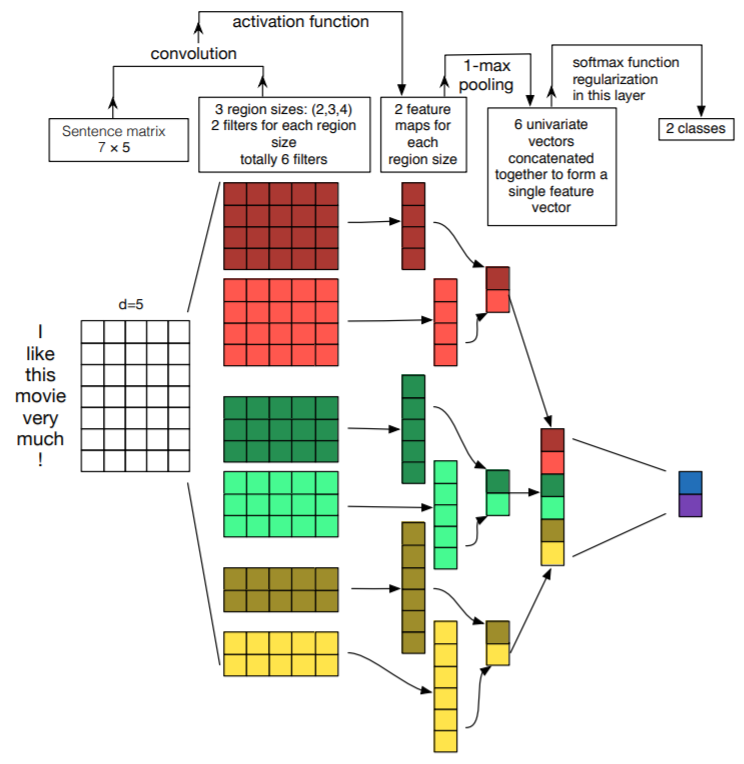
\includegraphics[width=0.6\textwidth]{Img/textcnn.png}
    \bicaption{一个用于句子分类的CNN结构表示}{Illustration of a CNN architecture for sentence classification}
    \label{fig:textcnn}
\end{figure}

\subsection{对话表示层设计}
分析来自聊天消息的对话是一项上层的文本挖掘任务,因为当理解一个句子时,它需要考虑对话范围内的上下文信息,因此针对对话级别的表示建模中,本文利用双向长期短期记忆网络(BiLSTM\cite{graves2013speech}),将对话的句子视为顺序序列,以捕获上下文信息,其中句子的表示由TextCNN表示。BiLSTM为序列学习任务编码双向信息,其堆叠两个方向相反的标准LSTM层,以分别学习句子的单向表示。然后,它将前向和后向表示形式组合为双向嵌入。LSTM是基于Hochreiter等人\cite{hochreiter1997long}提出的基于门机制的优化的递归神经网络(RNN)结构。LSTM利用门机制来提取关键信息,并将其传递给后面的长序列。LSTM单元由输入门,忘记门,单元状态和输出门组成。如图\ref{fig:lstm}(\subref{fig:lstm})所示为LSTM单元的模型结构。
\begin{figure}[htb]
    \centering
    \begin{subfigure}[b]{0.45\textwidth}
      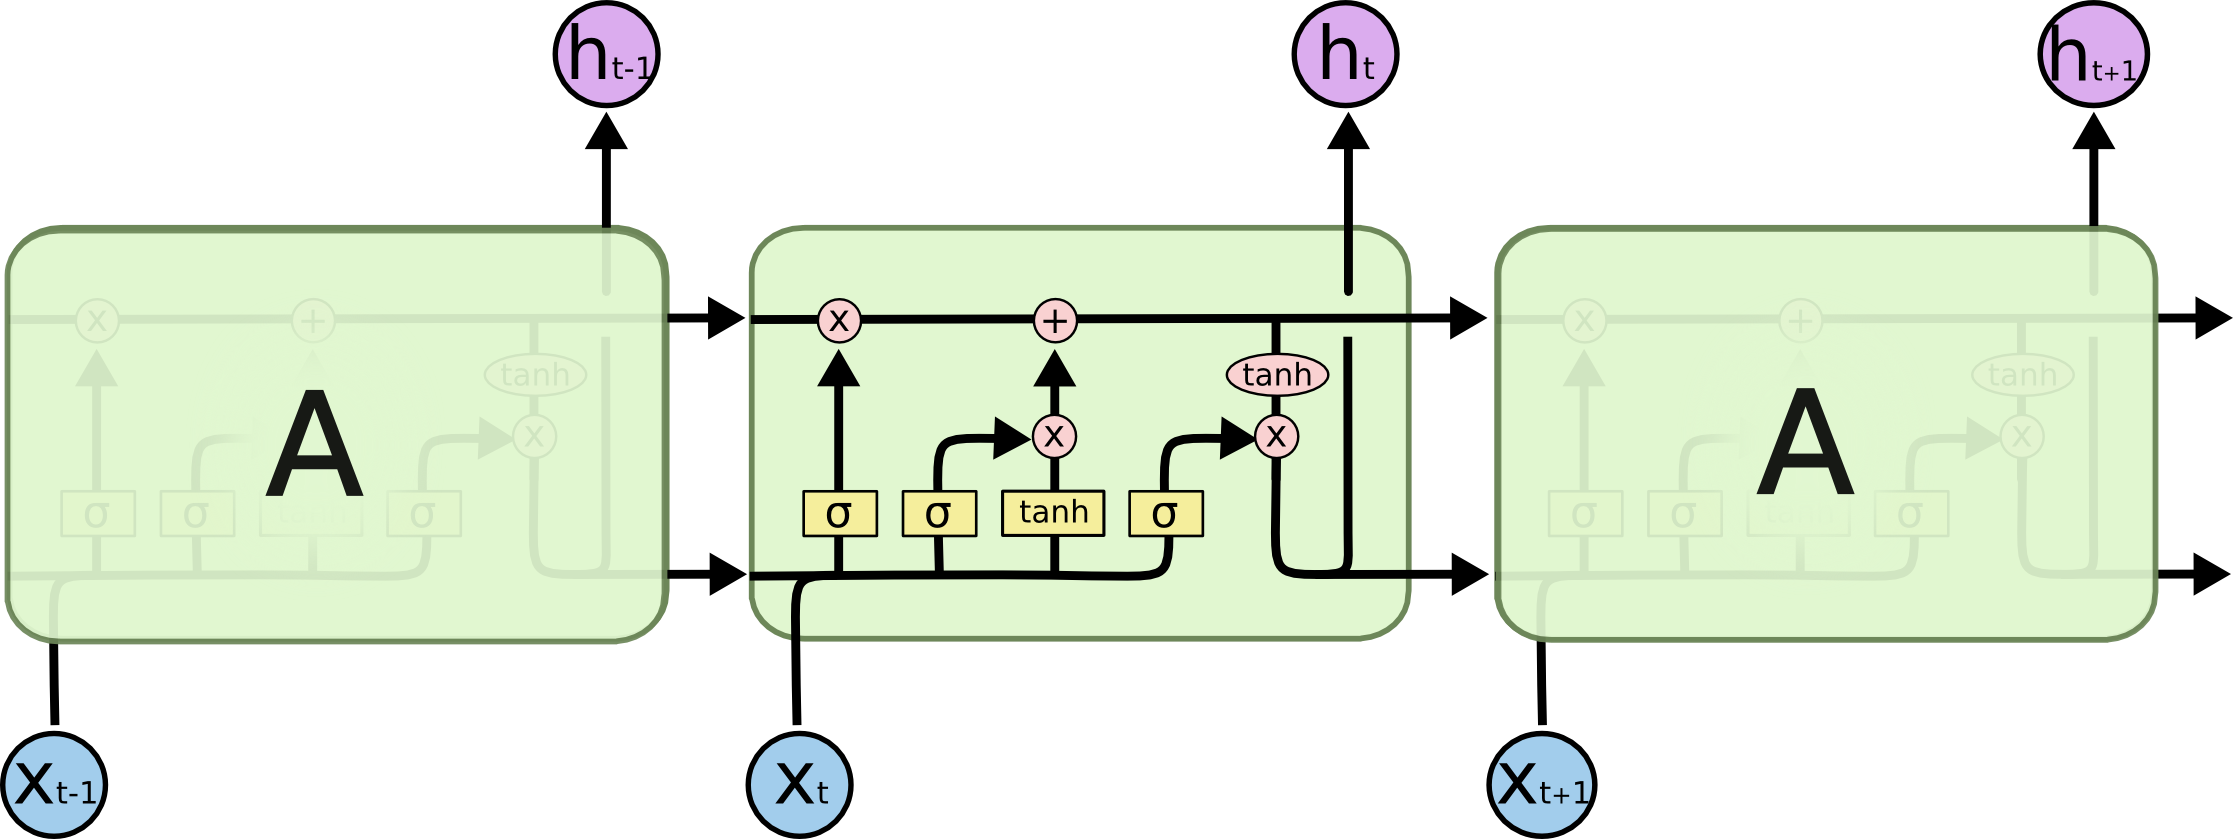
\includegraphics[width=\textwidth]{Img/lstm.png}
      \caption{}
      \label{fig:lstm}
    \end{subfigure}%
    ~% add desired spacing
    \begin{subfigure}[b]{0.45\textwidth}
      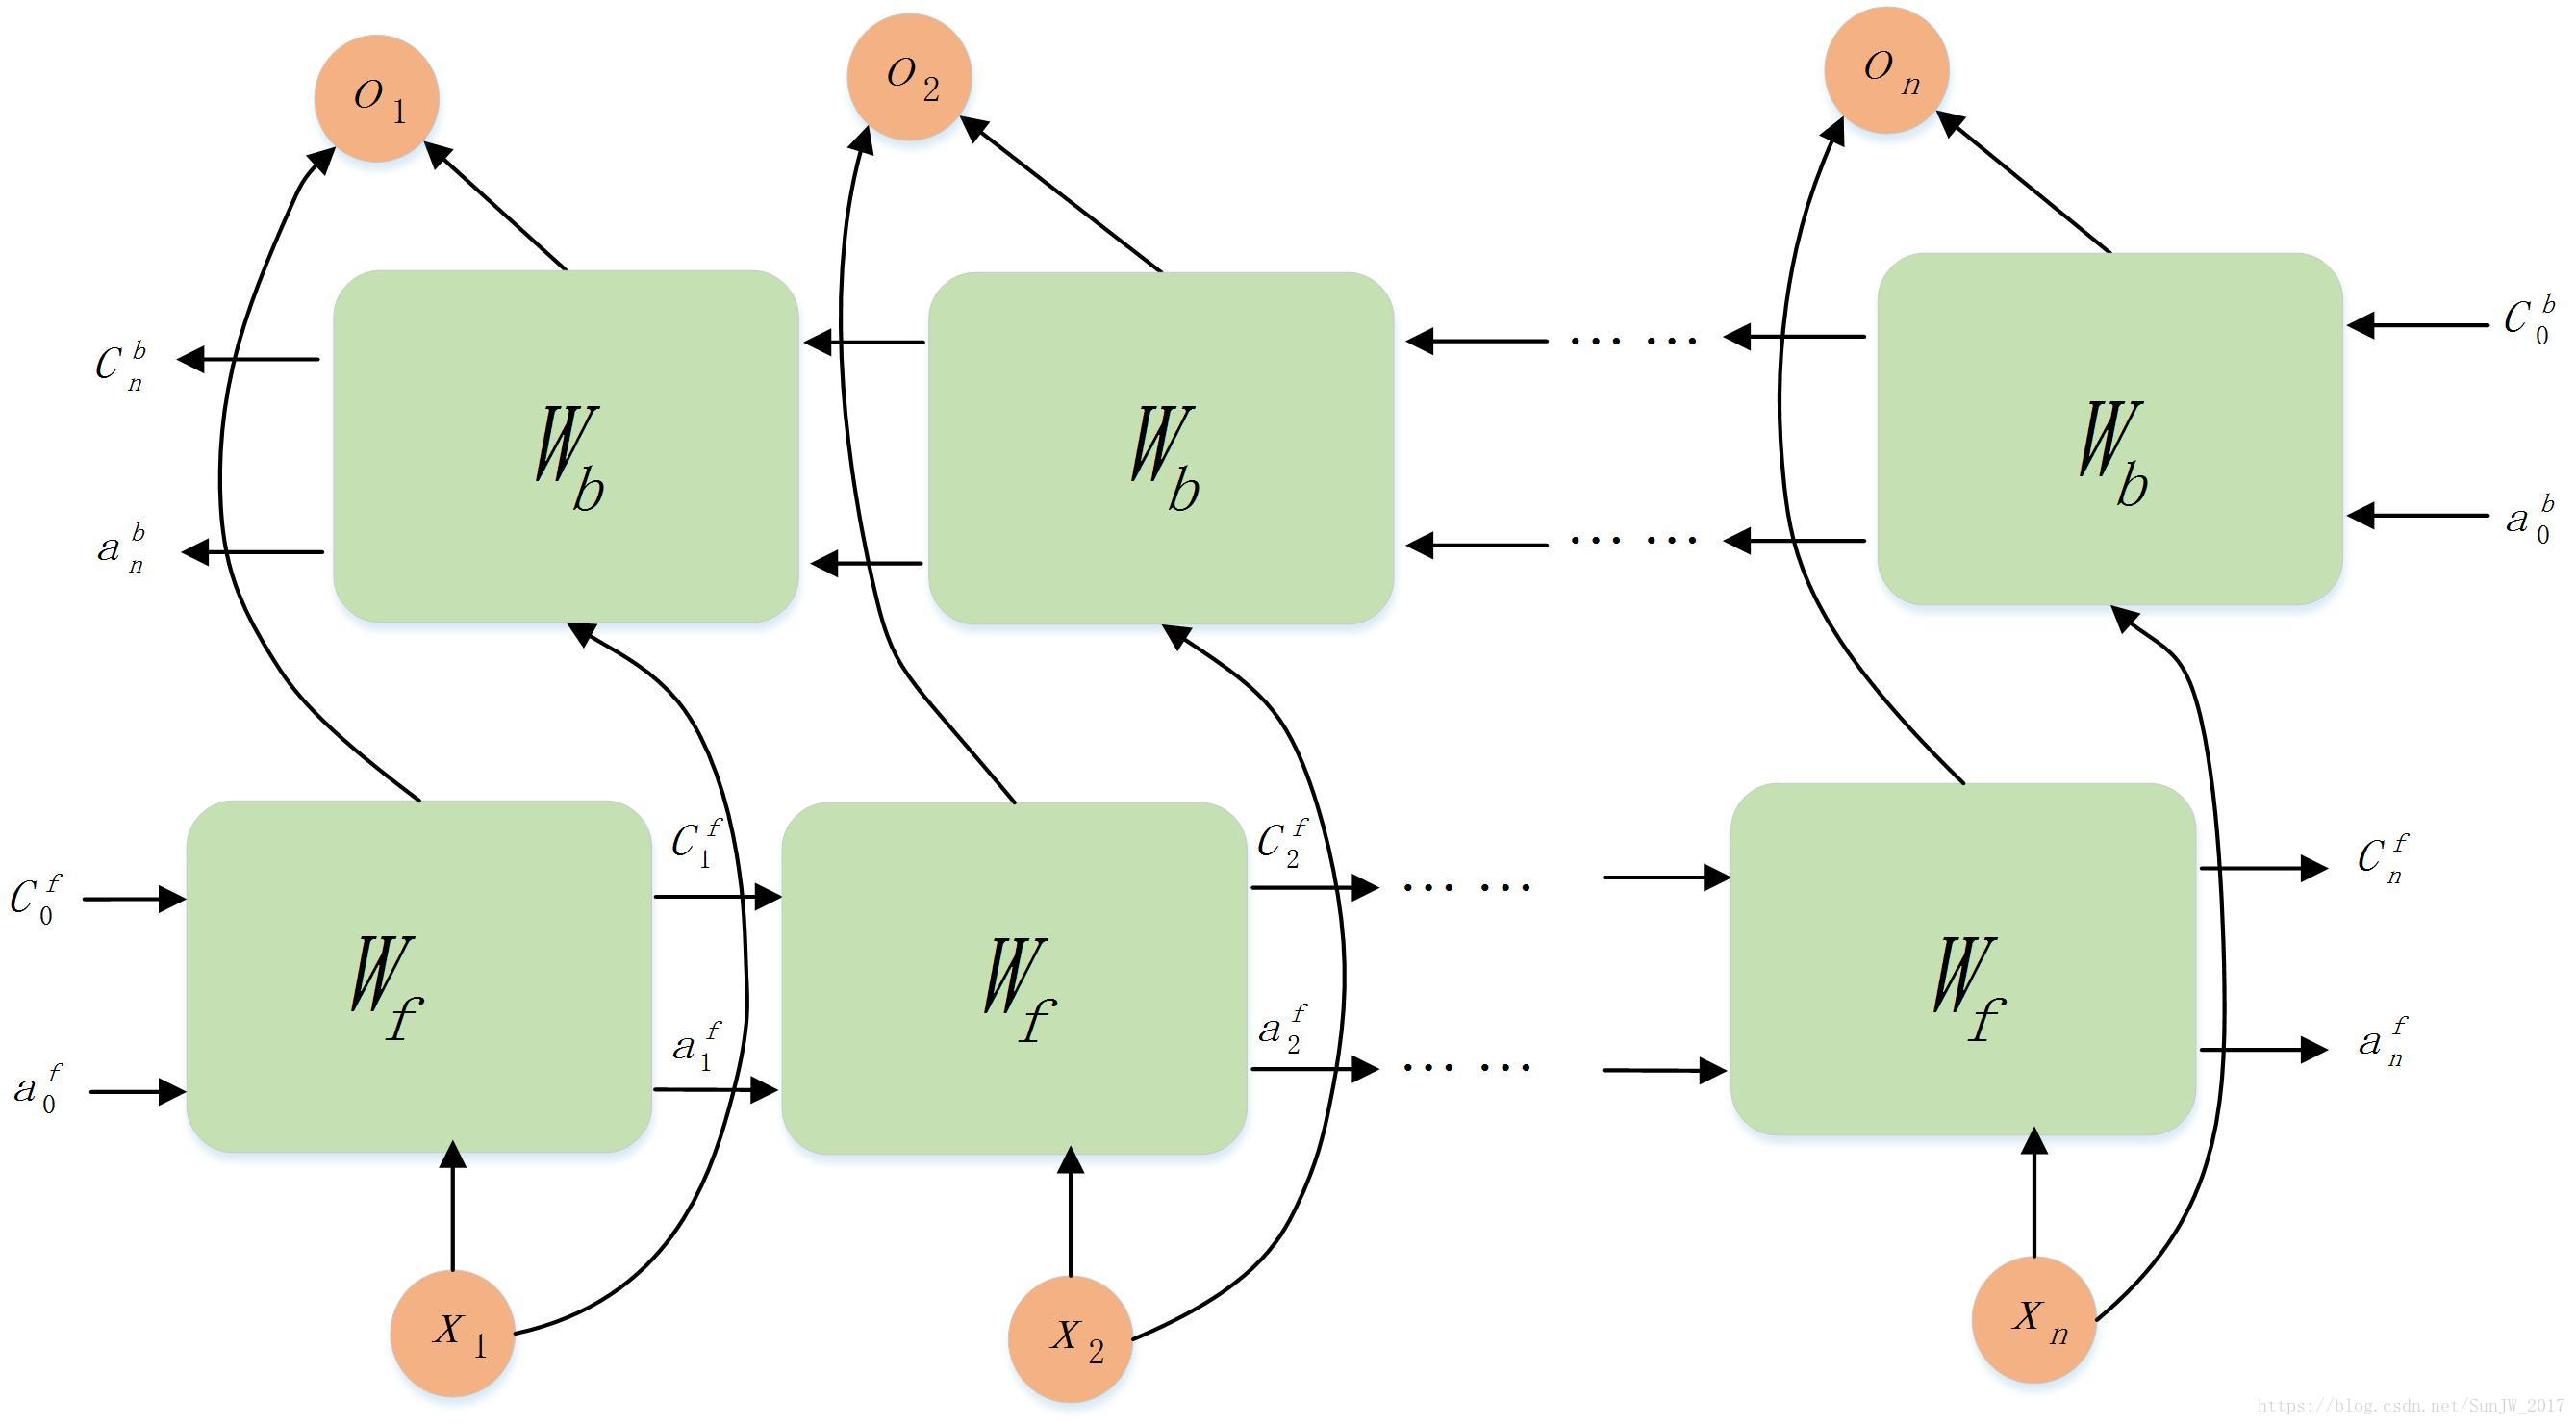
\includegraphics[width=\textwidth]{Img/bilstm.jpg}
      \caption{}
      \label{fig:bilstm}
    \end{subfigure}
    \bicaption{LSTM和BiLSTM结构。(a) 为LSTM结构,(b) 为BiLSTM,其使用两个LSTM}{The architectures of LSTM and BiLSTM. (a) LSTM structure, (b) BiLSTM structure, which uses two LSTM}
    \label{fig:lstm}
\end{figure}

% \begin{figure}[htb]
%     \centering
%     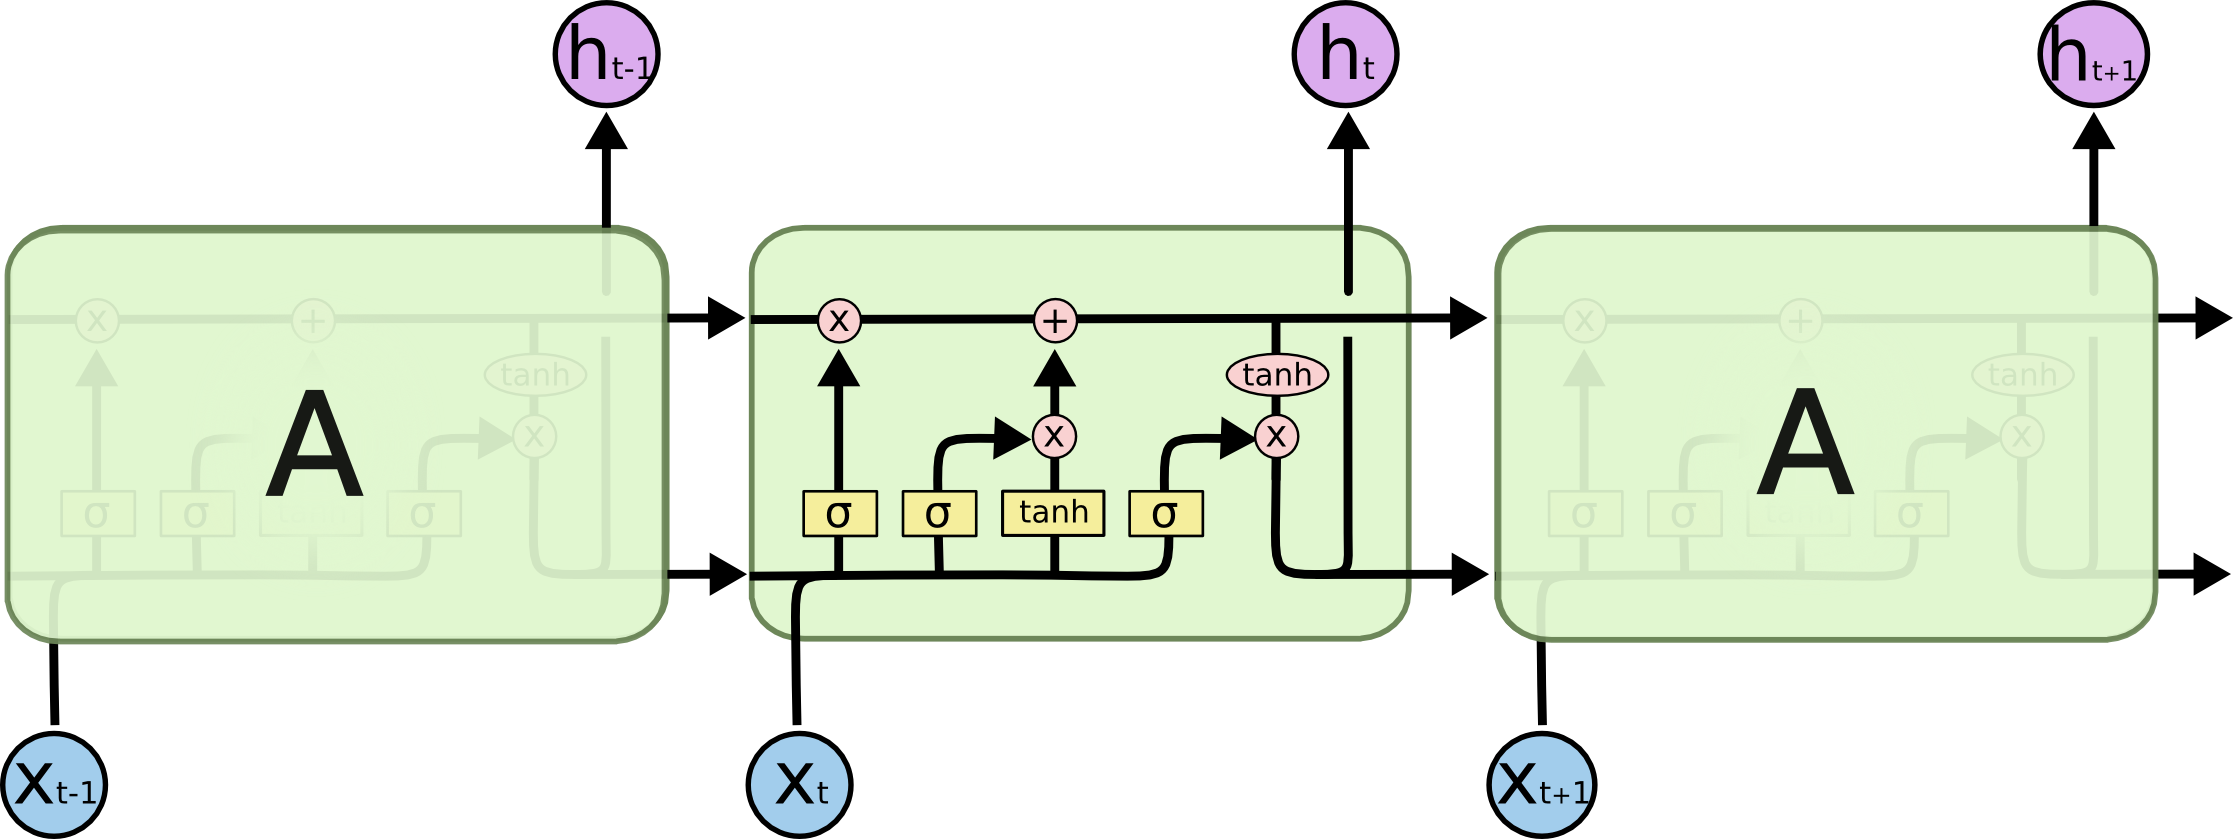
\includegraphics[width=0.6\textwidth]{Img/lstm.png}
%     \bicaption{一个LSTM单元的结构表示}{Illustration of an LSTM cell architecture}
%     \label{fig:lstm}
% \end{figure}
其中,LSTM单元门的输出可以表示如下:
$$\begin{aligned}\left[\begin{array}{c}{{\mathbf{i}_{t}} \\ {\mathbf{f}_{t}} \\ \tilde{\mathrm{c}}_{t}} \\ {\mathbf{o}_{t}}\end{array}\right] &=\left[\begin{array}{c}{\sigma} \\ {\sigma} \\ {tanh} \\ {\sigma}\end{array}\right] \left( \mathbf{W} \left[\begin{array}{c}{\mathbf{x}_{t}} \\ {\mathbf{h}_{t-1}}\end{array}\right] +\mathbf{b} \right)  \tag{1} \\ \mathbf{c}_{t} &=\tilde{\mathbf{c}}_{t} \odot \mathbf{i}_{t}+\mathbf{c}_{t-1} \odot \mathbf{f}_{t} \tag{2} \\ \mathbf{h}_{t} &=\mathbf{o}_{t} \odot \tanh \left(\mathbf{c}_{t}\right) \tag{3} \end{aligned}$$
其中$\mathbf{x}_{t}$ 是在这个输入句子中的第$i^{th}$个token,$\mathbf{W}$是LSTM单元的权重矩阵,$\mathbf{b}$是偏置项,$\mathbf{\sigma}$是sigmod激活函数,$\mathbf{tanh}$是双曲正切函数,$\odot$是element-wise的乘法。
因此,BiLSTM最终可表示为 $h=[\overrightarrow{h}\oplus \overleftarrow{h}]$,其中 $ \overleftarrow{h}$ 和  $ \overleftarrow{h}$分别表示两层LSTM的输出, $\oplus$ 表示连接运算。
如图\ref{fig:lstm}(\subref{fig:bilstm})所示为BiLSTM的结构示意图。
% \begin{figure}[htb]
%     \centering
%     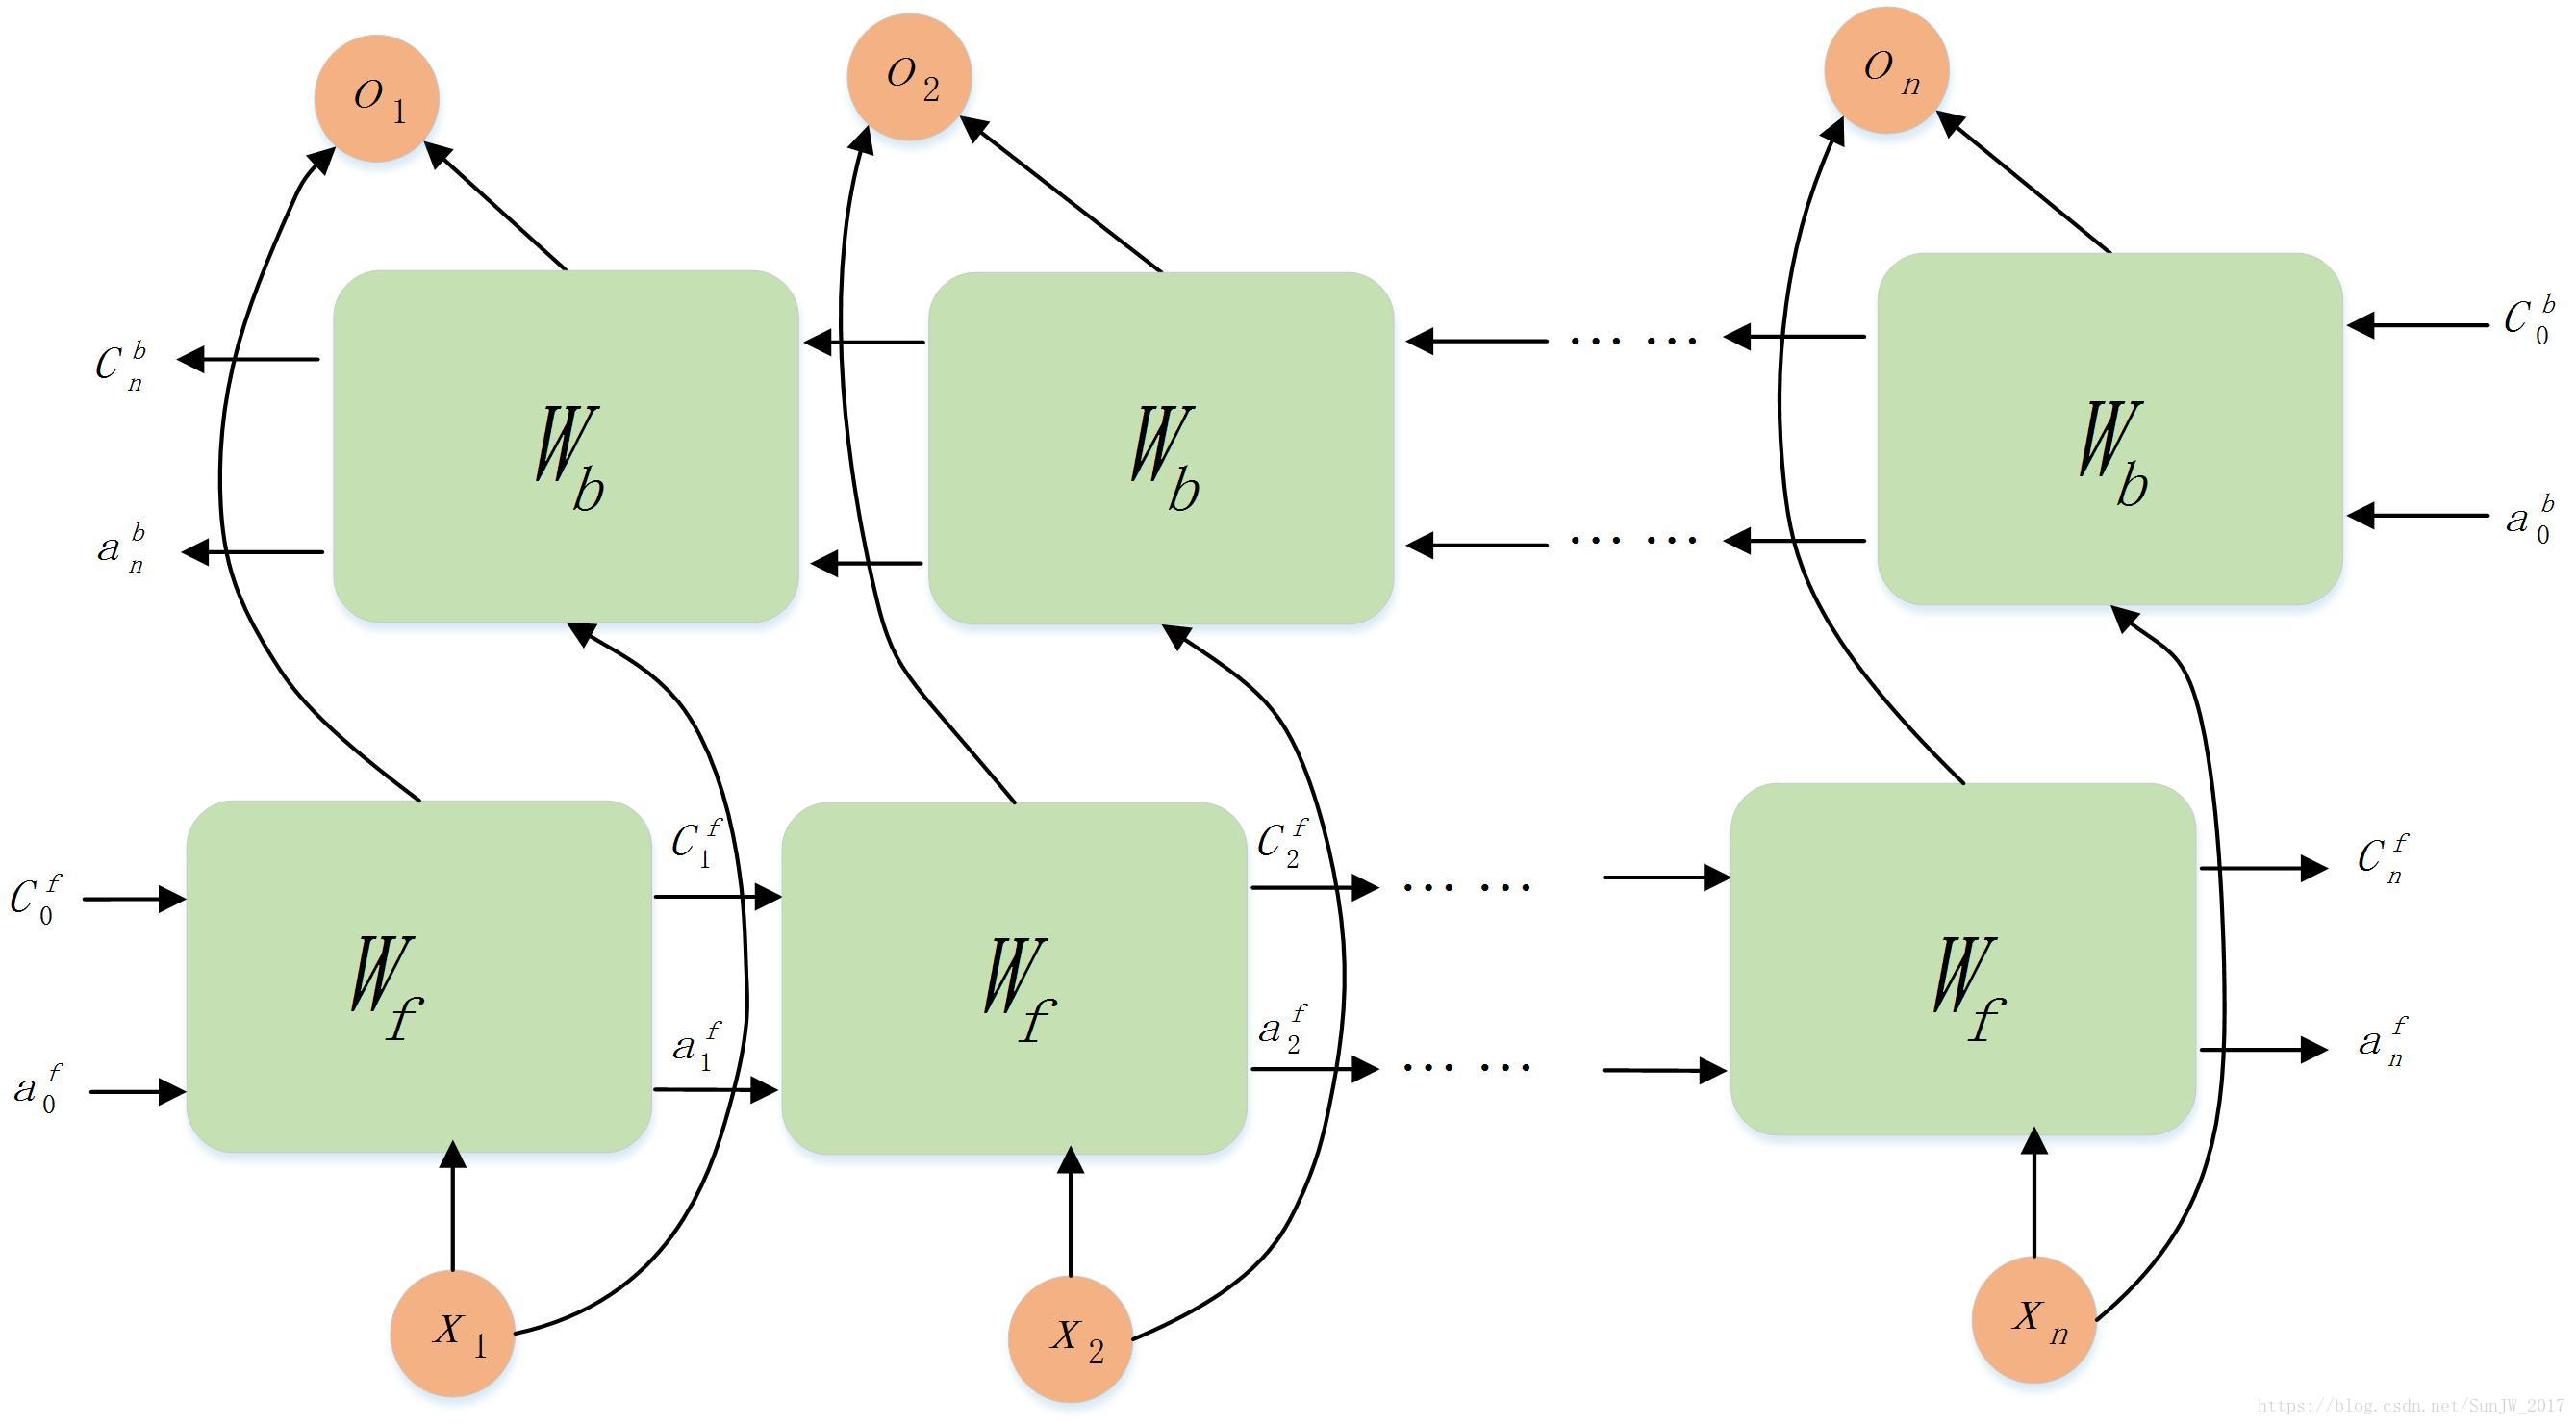
\includegraphics[width=0.4\textwidth]{Img/bilstm.jpg}
%     \bicaption{BiLSTM的结构表示}{Illustration of BiLSTM architecture}
%     \label{fig:bilstm}
% \end{figure}
本文使用一系列句子向量来表示对话,当把句子根据对话中的顺序输入BiLSTM编码器时,每个向量表达的句子都被当作基本单元。在对BiLSTM进行编码之后,可以学习对话的双向上下文信息。

\subsection{输出层设计}
\textbf{输出层:}在输出层中,本文组合由BiLSTM编码的两个方向表示$\overrightarrow{h}$和$\overleftarrow{h}$作为对话的输出向量,其可以表示为$h=[\overrightarrow{h}\oplus \overleftarrow{h}]$。

% \section{上下文敏感对话分类模型设计}
% 本文目的在于对从聊天记录中解耦得到的对话进行分类,并将对话分类为表示需求意图的对话和不是需求意图的对话,从而达到从聊天记录中进行隐藏需求对话识别的目的。为了清楚起见,在下文中,将使用\textit{feature dialog}和\textit{non-feature dialog}来表示需求意图的对话和不是需求意图的对话。

% 对话经过上下文敏感对话模型之后,在输出层可以得到对话对应的向量化表示,该向量化表示可以应用于如线性前馈网络等分类层从而进行文本分类。
% 本文构建了一个上下文敏感对话分类模型plain-{\tool},下文中使用p-{\tool}表示该模型。其模型结构图如图\ref{fig:model-cls}所示,模型是在前文所述的上下文敏感对话模型的基础上添加线性分类层,其可以对需求对话进行分类识别。
% \begin{figure}[htbp]
%     \centering
%     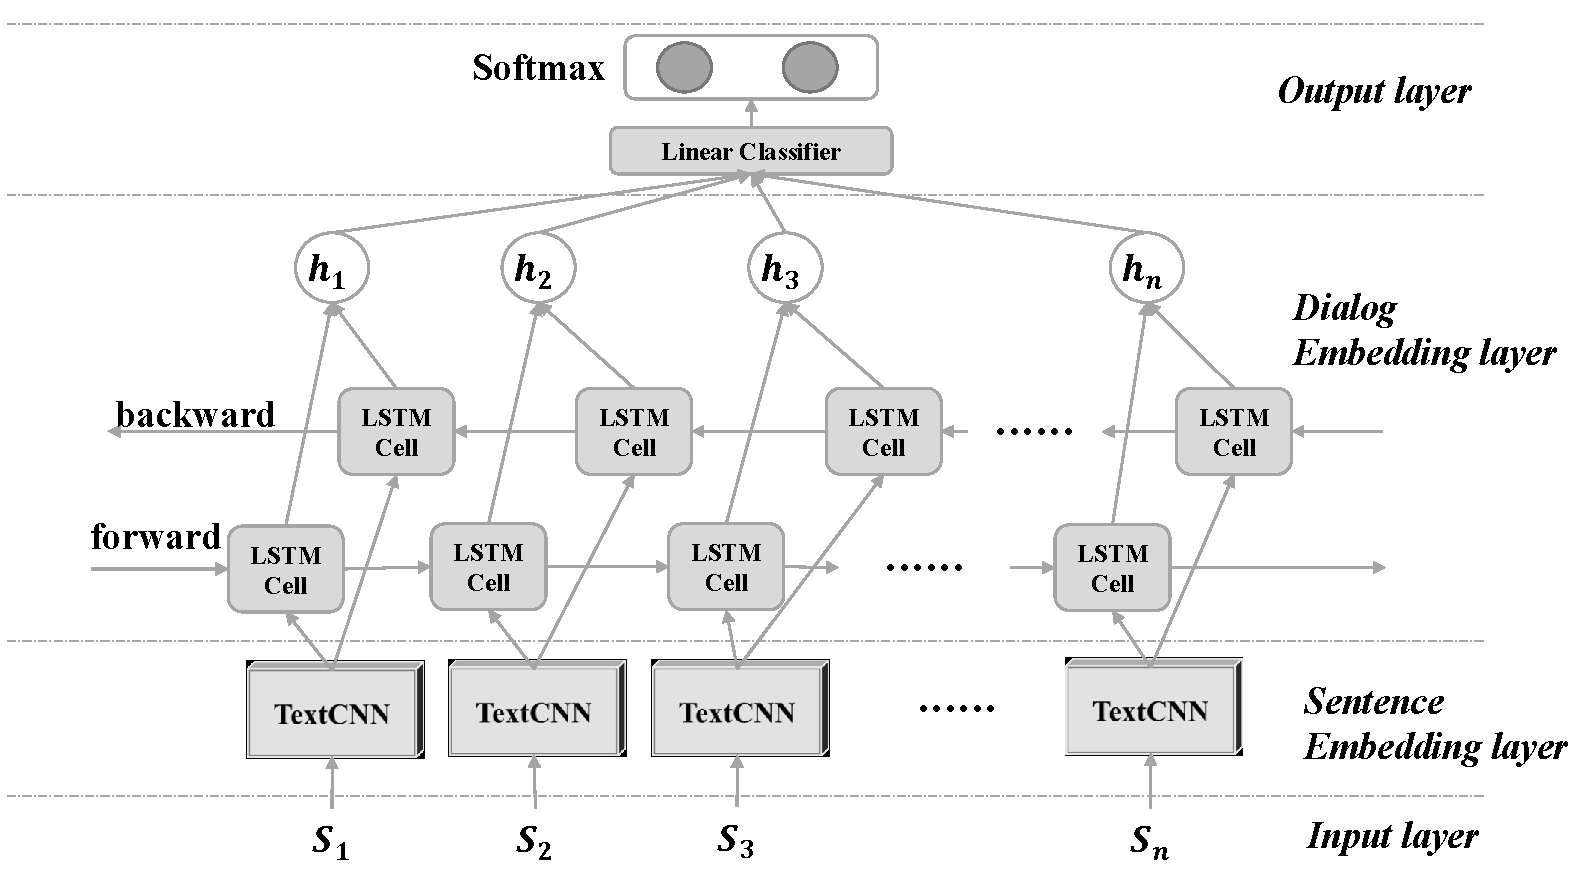
\includegraphics[width=\textwidth]{Img/model_cls.pdf}
%     \bicaption{p-{\tool}上下文敏感对话分类模型}{p-{\tool} Context-aware Dialog Classification Model}
%     \label{fig:model-cls}
% \end{figure}

% 由于每个对话都属于\textit{feature dialog}类或\textit{non-feature dialog}类,因此分类层输出为长度为2的向量$[score_1 , score_2]$  ,代表两个类的分数,其中$score_i \in \mathbb{R}$ 。 接下来对此向量执行softmax,表示为
% $$Softmax(socre_i)=\frac{e^{score_i}}{\sum_{j=1}^2 e^{score_j}}$$ 
% ,可以将 $[score_1 , score_2]$ 归一化为概率$[p ,1-p]$,其中 $p \in [0,1]$。

% \section{上下文敏感对话模型实现}

% 在模型实现部分,p-{\tool}使用AllenNLP\footnote{https://allennlp.org/},一个基于PyTorch\footnote{https://pytorch.org/}构建的开源NLP库来进行实现。

% 在代码实现上下文敏感对话模型结构时,主要继承AllenNLP的\textit{Model}类,其实现了NLP中一些常见的方法,如Vocabulary中word到index的映射、参数初始化、正则项等,这些方法可以为{\tool}的实现减少大量的重复工作。

% 对于训练过程,主要继承了AllenNLP的\textit{Trainer}类,其实现了一些神经网络训练过程中常用的方法,如序列化保存、GPU训练、数据集加载、梯度裁剪、TensorBoard可视化等。训练过程中所需要的参数保存在json文件中,AllenNLP加载json文件并初始化\textit{Trainer}类,然后开始进行训练以及评估测试。

% 对于超参数,本文选用Grid Search\cite{Bergstra2012Random}作为参数选择方法以获得最佳效果。pos-tag向量的维度为50,与单词向量相同。然后,可以使用$s=[w_1,w_2\dots w_n]$ 作为句子的表示形式,其中$w_i=[we_i\oplus pos_i]$。为了获得由不同尺度的局部信息组合而成的更充分的语义信息,本文对句子应用具有不同大小的多个卷积核,其大小分别是2、3、4、5,每类卷积核有25个。BiLSTM的输出维度为300(每个方向是150维)。由于该任务可以视为分类问题,因此本文将交叉熵用作损失函数。

% 此外,为避免过拟合问题,本文以0.1的dropout rate对输入向量进行Dropout \cite{srivastava2014dropout},这意味着将随机屏蔽10%的神经元以减少每次批量训练中需要训练的参数。本文还使用了Early Stopping\cite{prechelt1998early}的策略,如果测试数据集的效果在10个Epoch内未提升,则训练过程将停止。对于神经网络的优化器,由于Adam\cite{kingma2014adam}对梯度的一阶矩估计和二阶矩估计进行综合考虑,并且其具有自适应性能好、参数的更新不受梯度的伸缩变换影响等特点,本文使用Adam优化器对模型参数进行更新优化。

\section{本章小结}

本章介绍了对话解耦这一对流式聊天记录进行对话信息必不可少的步骤,以及本文中使用的对话解耦模型。接下来介绍通过分层的、分别使用TextCNN和BiLSTM对句子和对话级别进行语义表示的上下文敏感对话模型{\dm},该模型可以将对话转换为向量化表示,该向量嵌入了对话的语义信息,并使该对话信息应用到下文中的需求识别任务中。
% 另外,针对上下文敏感对话模型,本章构建了p-{\tool},该模型通过增加线性分类层可以对对话进行分类,从而达到需求识别的目的。最后,介绍了p-{\tool}的模型实现相关细节。

\chapter{基于孪生网络的隐藏需求挖掘方法}
% 上文中介绍的p-{\tool}可以对单个对话进行建模并进行分类,但由于数据标注困难的问题,p-{\tool}模型存在着训练数据不足的问题。针对这个问题,
本章介绍了本文设计的{\tool}方法,其总体框架如图\ref{fig:approach}所示,{\tool}以第3章中设计的两个相同上下文敏感对话模型为基模型构建了一个孪生网络,并构建Pair-Instance作为{\tool}的输入样本,分类目标为输入的两个对话是否为相同的类别。在获取{\tool}对输入的两个对话是否为相同类别的预测之后,{\tool}基于此预测结果和配对实例中已标注对话的实际标签来推断目标对话的预测类别,以达到对对话进行分类的目的,从而可以进行需求识别。
\begin{figure}[htbp]
    \centering
    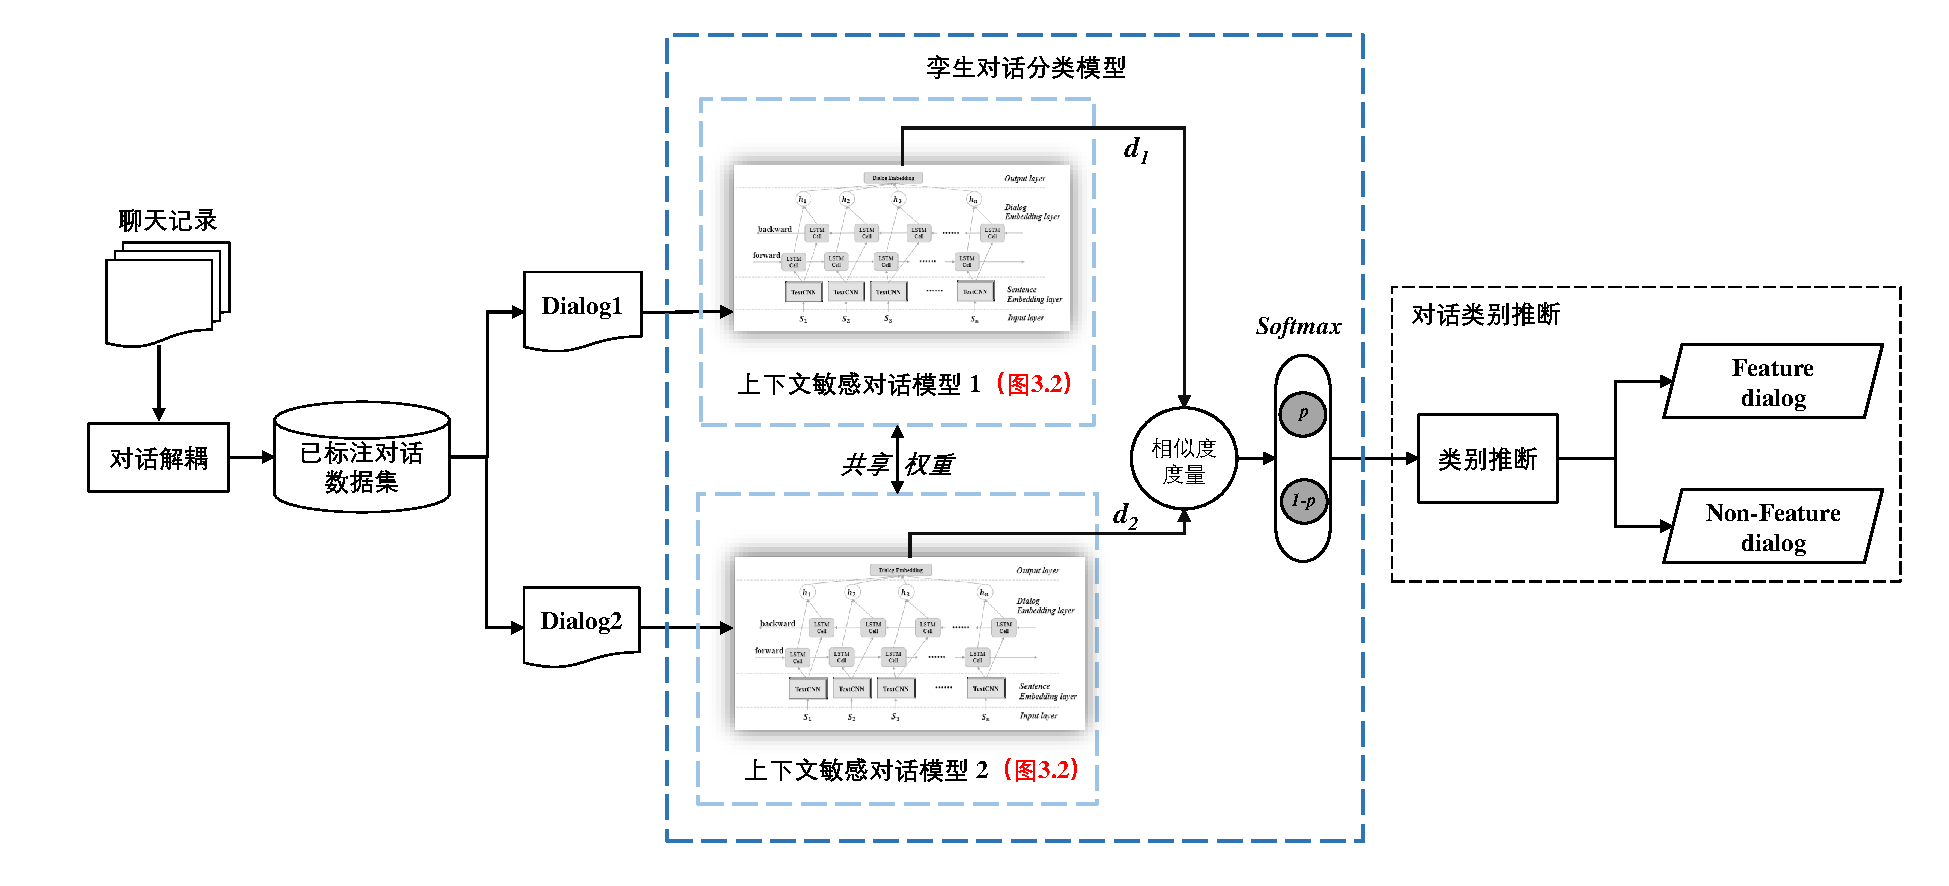
\includegraphics[width=\textwidth]{Img/approach.pdf}
    \bicaption{FRMiner模型结构图}{Architecture of FRMiner}
    \label{fig:approach}
\end{figure}


\section{{\tool}模型结构设计}
为了缓解标注数据不足的问题,本文构建了对话分类孪生网络,传统的文本分类方法将单个对话映射到其类别,本文则将其转换为确定两个对话是否属于同一类的任务,同时可以扩充数据集。为了清楚起见,在下文中,将使用\textit{feature dialog}和\textit{non-feature dialog}来表示为需求意图的对话和不是需求意图的对话。

图\ref{fig:approach}中标识Siamese Dialog Classification Network的虚线框显示了孪生网络详细的体系结构,对话分类孪生网络包含两个上下文敏感对话模型,它们共享结构和参数,并将一对对话分别编码为$d_1$和$d_2$。本文使用$d_1$和$d_2$的组合形式$[{d_1}\oplus {d_2}]$来表示两个对话之间的关系。然后将一对对话之间关系的表示映射为相似度度量值。由于常见的用于相似度度量的显式函数(例如余弦相似度和欧几里得距离\cite{huang2008similarity})通常用于测量线性空间中向量之间的接近度,而并不适用于衡量语义空间中的复杂对话相似性。本文选择采用在训练神经网络过程中学习到的相似性函数。由于可以获得两个对话是否相似的标签,因此可以据此标签和对话输入训练神经网络中的相似层,它就像一个黑匣子模块,输入是带有\textit{same}或\textit{diff}标签的两个对话的向量式表示,输出是它们的相似性。

本文按照以下步骤训练对话分类孪生网络。
\begin{enumerate}
    \item 首先将数据集随机分为训练和测试数据集。\textit{Train\_d}是原始数据集,它使用带有标签\textit{feature dialog}或\textit{non-feature dialog}的对话作为基本数据单元。
    \item 由于标注对话的大小不足以训练有效的基于有监督学习的模型,为了解决该问题,本文通过采样来自\textit{Train\_d}的一对对话作为\textit{Train\_p}(标签为\textit{same}或\textit{diff})的一个基本数据单元,并将\textit{Train\_d}数据集增强为\textit{Train\_p}。更具体地说,对于训练数据集中的每个对话,本文从训练数据集\textit{Train\_d}中分别随机选择一个带有\textit{feature dialog}标签的正样本和一个带有\textit{non-feature dialog}标签的负样本。例如,如果两个对话都是\textit{feature dialog}或\textit{non-feature dialog},将为它们分配标签\textit{same},否则为\textit{diff}。由于采用一正一负的抽样策略,训练数据可以天然地进行数据平衡。此外,假设在\textit{Train\_d}中有 $m$ 个需求对话和$n$个非需求对话,在\textit{Train\_p}可以将原始数据集扩展为 $\tbinom{m}{2}+\tbinom{n}{2}+m\times n$。但是此种数据增强方式获得的数据量过大,为了减小数据增强后的数据集规模,同时又不能增大随机采样带来的误差,本文对以上流程在整个数据集上及进行$iter\_num$次。伪代码如算法\ref{alg:trainset}所示:
    \begin{algorithm}[htb]
            \caption{FRMiner Pair-Instance训练集构建算法}  
            \label{alg:trainset}
            \begin{algorithmic}[1]
                \Require list 正样本集合 Pos,list 负样本集合 Neg, int 迭代次数 iter\_num 
                \Ensure list <pair> 训练集 
                \Function{pair\_instance}{list Pos, list Neg, int iter\_num} 
                    \State pairs \gets [\ ]
                    \For {i\ in\ range(iter\_num)}
                        \For {d\ \in\ Pos\ \cup\ Neg}
                            \State p \gets random(Pos)
                            \State n \gets random(Neg)
                            \State pairs.append(<d,\ p>)
                            \State pairs.append(<d,\ n>)
                        \EndFor
                    \EndFor
                    \State \Return $pairs$
                \EndFunction  
            \end{algorithmic}  
    \end{algorithm}
    \item 最后,由于每对对话都属于\textit{same}类或\textit{diff}类,因此相似性度量的输出为长度为2的向量$[score_1 , score_2]$  ,代表两个类的分数,其中$score_i \in \mathbb{R}$ 。 接下来对此向量执行softmax,表示为
$$Softmax(socre_i)=\frac{e^{score_i}}{\sum_{j=1}^2 e^{score_j}}$$ 
    ,可以将 $[score_1 , score_2]$ 归一化为概率$[p ,1-p]$,其中 $p \in [0,1]$。
\end{enumerate}


\section{对话分类概率推断}
对话分类孪生网络的输出是表示两个对话是相似还是不相似的概率。但是本文需要的是目标对话是否为需求对话的概率,因此需要基于对话相似的概率和配对对话的实际标签来推断此对话的标签。例如,首先采样一对$<Dialog_1,Dialog_2>$ ,其中 $Dialog_1$ 是从训练数据集中采样的有标签对话,其标签为\textit{non-feature dialog},而 $Dialog_2$是要预测的未知对话。然后将它们输入到对话分类孪生网络中,然后做出两个对话为相似或不相似的预测。假设预测为不相似,则可以推断出$Dialog_2$ 的类为\textit{feature dialog}。如果$Dialog_2$ 的实际标签是\textit{feature dialog},则表明模型做出的这种预测是正确的。否则,预测结果是假阳的。伪代码如算法\ref{alg:infer}所示:
    \begin{algorithm}[!htb]
            \caption{测试阶段分类类别Inference算法}  
            \label{alg:infer}
            \begin{algorithmic}[1]
                \Require list 训练样本集 train,list 测试样本集 test
                \Function{test\_infer}{list train, list test} 
                    \For{t\ in\ test}
                    \State golden \gets random(train)
                    \State p \gets FRMiner(<t,\ golden>)
                    \If {p\ is\ 'same'}
                        \If {golden.label\ is\ 'feature'}
                        \State t.label \gets 'feature'
                        \EndIf
                        \If {golden.label\ is\ 'non-feature'}
                        \State t.label \gets 'non-feature'
                        \EndIf
                    \EndIf
                    \If {p\ is\ 'diff'}
                        \If {golden.label\ is\ 'feature'}
                        \State t.label \gets 'non-feature'
                        \EndIf
                        \If {golden.label\ is\ 'non-feature'}
                        \State t.label \gets 'feature'
                        \EndIf
                    \EndIf
                    \EndFor
                \EndFunction  
            \end{algorithmic}  
    \end{algorithm}
    
为了获得更可靠的预测结果,本文在预测阶段时采用了投票策略。对于每个未知标签对话,本文通过对$k$个不同的有标签对话进行采样来构造$k$个配对样本。将这些对传递到FRMiner后,基于FRMiner的预测结果和有标签对话的标签,可以得到$l$个样本指示未知标签对话为\textit{feature dialog}和$k-l$个样本指示未知标签对话为\textit{non-feature dialog}。如果$l$大于$\frac{k}{2}$,则为预测的对话标注为\textit{feature dialog}标签,反之亦然。

\section{{\tool}模型实现细节}
本文的{\tool}模型代码以及数据已在\href{https://github.com/FRMiner/FRMiner}{https://github.com/FRMiner/FRMiner}开源,并提供有详细代码使用文档,使用者可运行代码对未标注对话进行需求识别或者基于代码做进一步研究。

对于模型实现,{\tool}使用了AllenNLP\footnote{https://allennlp.org/},一个基于PyTorch\footnote{https://pytorch.org/}构建的开源NLP库。

在实现{\tool}的模型结构时,主要继承AllenNLP的\textit{Model}类,其实现了NLP中一些常见的方法,如Vocabulary中word到index的映射、参数初始化、正则项等,这些方法可以为{\tool}的实现减少大量的重复工作。

不同于传统的单文本目标分类任务,孪生网络使用两个相同结构、共享参数的编码器对文本进行embedding,然后使用相似度度量层对Pair-Instance进行相似性评估。本研究对此并没有在代码中实现两个相同的网络,而是将两个对话分别输入到同一个上下文敏感对话模型中得到两个对话的embedding表示。在得到Pair-Instance的两个向量化表示之后,将其拼接为$[{d_1}\oplus {d_2}]$,其为一个300维向量,表示一对对话之间的关系。
然后本文使用线性层作为相似性度量层,将这个300维向量映射到两个值,这些值表示两个类别的概率得分。同样的,由于该任务可以视为分类为\textit{same}和\textit{diff}的二分类问题,因此本文将交叉熵用作损失函数。

对于训练过程,主要继承了AllenNLP的\textit{Trainer}类,其实现了一些神经网络训练过程中常用的方法,如序列化保存、GPU训练、数据集加载、梯度裁剪、TensorBoard可视化等。训练过程中所需要的参数保存在json文件中,AllenNLP加载json文件并初始化\textit{Trainer}类,然后开始进行训练以及评估测试。

对于超参数,本文选用Grid Search\cite{Bergstra2012Random}作为参数选择方法以获得最佳效果。pos-tag向量的维度为50,与单词向量相同。然后,可以使用$s=[w_1,w_2\dots w_n]$ 作为句子的表示形式,其中$w_i=[we_i\oplus pos_i]$。为了获得由不同尺度的局部信息组合而成的更充分的语义信息,本文对句子应用具有不同大小的多个卷积核,其大小分别是2、3、4、5,每类卷积核有25个。BiLSTM的输出维度为300(每个方向是150维)。

此外,为避免过拟合问题,本文以0.1的dropout rate对输入向量进行Dropout \cite{srivastava2014dropout},这意味着将随机屏蔽10%的神经元以减少每次批量训练中需要训练的参数。本文还使用了Early Stopping\cite{prechelt1998early}的策略,如果测试数据集的效果在10个Epoch内未提升,则训练过程将停止。对于神经网络的优化器,由于Adam\cite{kingma2014adam}对梯度的一阶矩估计和二阶矩估计进行综合考虑,并且其具有自适应性能好、参数的更新不受梯度的伸缩变换影响等特点,本文使用Adam优化器对模型参数进行更新优化。




\section{本章小结}

本章主要针对{\tool}介绍其构建过程、模型结构、针对Pair-Instance的目标对话类别推断以及模型细节和应用部署进行介绍。首先,本文使用孪生网络拼接两个相同结构、共享参数的上下文敏感对话模型,针对Pair-Instance进行分类,最后针对目标对话使用类别推断获取其预测标签。最后,本章介绍了模型配置细节以及训练中的参数调优。
\chapter{需求对话识别模型验证与分析}
本章目的在于对模型参数进行定量分析、通过把FRMiner与近年先进的需求识别基准方法和常见文本分类模型的效果对比验证孪生网络在复杂对话分类中的有效性以及FRMiner在跨项目实验中的表现,并分别介绍了以上实验的设置和实验结果说明和基本分析。

\section{验证实验设计}
这部分主要介绍我们设计的三个实验以及实验的基本设置。这三个实验都从三个开源项目数据集上使用了三折交叉验证\cite{DBLP:conf/ijcai/Kohavi95}。首先,我们随即将我们的数据集分成三部分,并使用其中两份作为训练集,剩下的一份作为测试集。我们重复这个过程三次,并且每次使用剩下的不同部分作为测试集。在三个实验中,均使用相同的分割数据集。另外,实验环境为Ubuntu操作系统,硬件配置为Intel core i7 CPU,16G RAM,NVIDIA 1060 GPU。
\subsection{FRMiner进行需求识别的有效性实验}
为了验证我们方法的有效性,我们针对从三个开源项目的聊天记录中进行特征请求对话识别实验进行了三折交叉验证。并且针对两个近年效果先进的在句子级别上分类为特征请求或者其他类别的分类器,我们与其比较了分类表现。由于原分类器的分类目标是句子,我们需要将其调整为对话级别的分类器,也即对话中包含为分类器预测为特征请求的句子时,我们认为该对话为特征请求对话。另外,我们和四个广泛使用的文本分类方法,进行对比,以验证FRMiner在有限标注数据上进行自动特征请求对话识别的有效性。

前面我们介绍了近年软件工程领域在特征请求识别方面的研究工作,其中章节2.1中的CNN-based Classifier(CNC)\cite{Huang2018Automating}和Feature Request Analyser(FRA) \cite{shi2017understanding}在特征请求分类上达到较好的效果。我们选用其作为特征请求分类方面的基线方法。CNC是目前从在线问题报告的评论中进行句子分类的最优模型,其使用基于卷积神经网络的方法把句子分为七个类别:信息提供、信息寻找、特征请求、问题提出、问题发现、方面验证和无意义的语句。我们使用其中特征请求的类别来预测,即将包含特征请求句子的对话分类为特征请求对话。FRA是一个从在线问题追踪系统中把句子进行特征请求分类的最优的基于规则的模型,其使用81个规则将句子分为六个类别,我们及那个包含类别\textit{Intent}的句子的对话分类为特征请求对话,同时,不包含\textit{Intent}句子的对话为非特征请求对话。对于CNC和FRA,我们使用了对应文献中中提供的代码和模型。

四个基于机器学习的方式我们选用如章节2.4.5中所述的朴素贝叶斯(NB)\cite{mccallum1998comparison}、随机森林(RF)\cite{liaw2002classification}、梯度提升决策树(GBDT)\cite{ke2017lightgbm} 和FastText(FT)\cite{joulin2016bag} 作为基线方法。NB为一个简单的使用词袋模型和贝叶斯规则的文本分类模型,它通过先验概率和学习训练数据得到的条件概率得到句子的后验概率,也即,给定一个句子,它可以推断出句子在所有类别下的概率。RF是一个使用多个树构建的集成机器学习模型,每个树都为最后的分类结果做贡献。在训练RF时,我们设置树的最大深度为2。GBDT是另一个集成学习方法,和RF的不同在于它的树是通过前面树的残差来决定的。当训练GBDT时,我们设置初始学习率为1.0,树的最大深度为1。FT是基于一个结构上类似于word2vec的浅层神经网络的文本分类方法,我们在实验中训练100轮,并设置初始学习率为1.0,输入n-gram的窗口大小为2。对于四个文本分类模型,我们使用官方提供的包 \footnote{https://scikit-learn.org/stable/} \footnote{https://fasttext.cc/},并且提取了词频-逆文档频率(TFIDF)\cite{joachims1996probabilistic} 作为对话特征向量来进行对话文本分类。接下来,我们使用网格搜索来微调四个文本分类模型的参数,使其达到最优效果。
另外,在以上的基线模型中,我们均使用了随机上采样\cite{ling1998data}来解决数据集的类别不均衡问题。

\subsection{孪生网络在FRMiner中的有效性实验}
为了检验引入孪生网络而带来的效果提升,我们构建了p-FRMiner,其是一个3.1中构建的以Single-Instance为输入的基本上下文敏感对话分类模型。然后,我们将p-{\tool}和使用Pair-Instance作为输入的{\tool}进行效果对比。之后,我们逐渐增加Pair-Instance训练集的大小来检验模型效果提升和数据集增强的关系。

需要注意的是,p-{\tool}和{\tool}是不同的分类模型,其中,p-{\tool}是对话上下文敏感模型,并接受单个对话作为输入,其模型结构图如图\ref{fig:model}所示。
\begin{figure}[htbp]
    \centering
    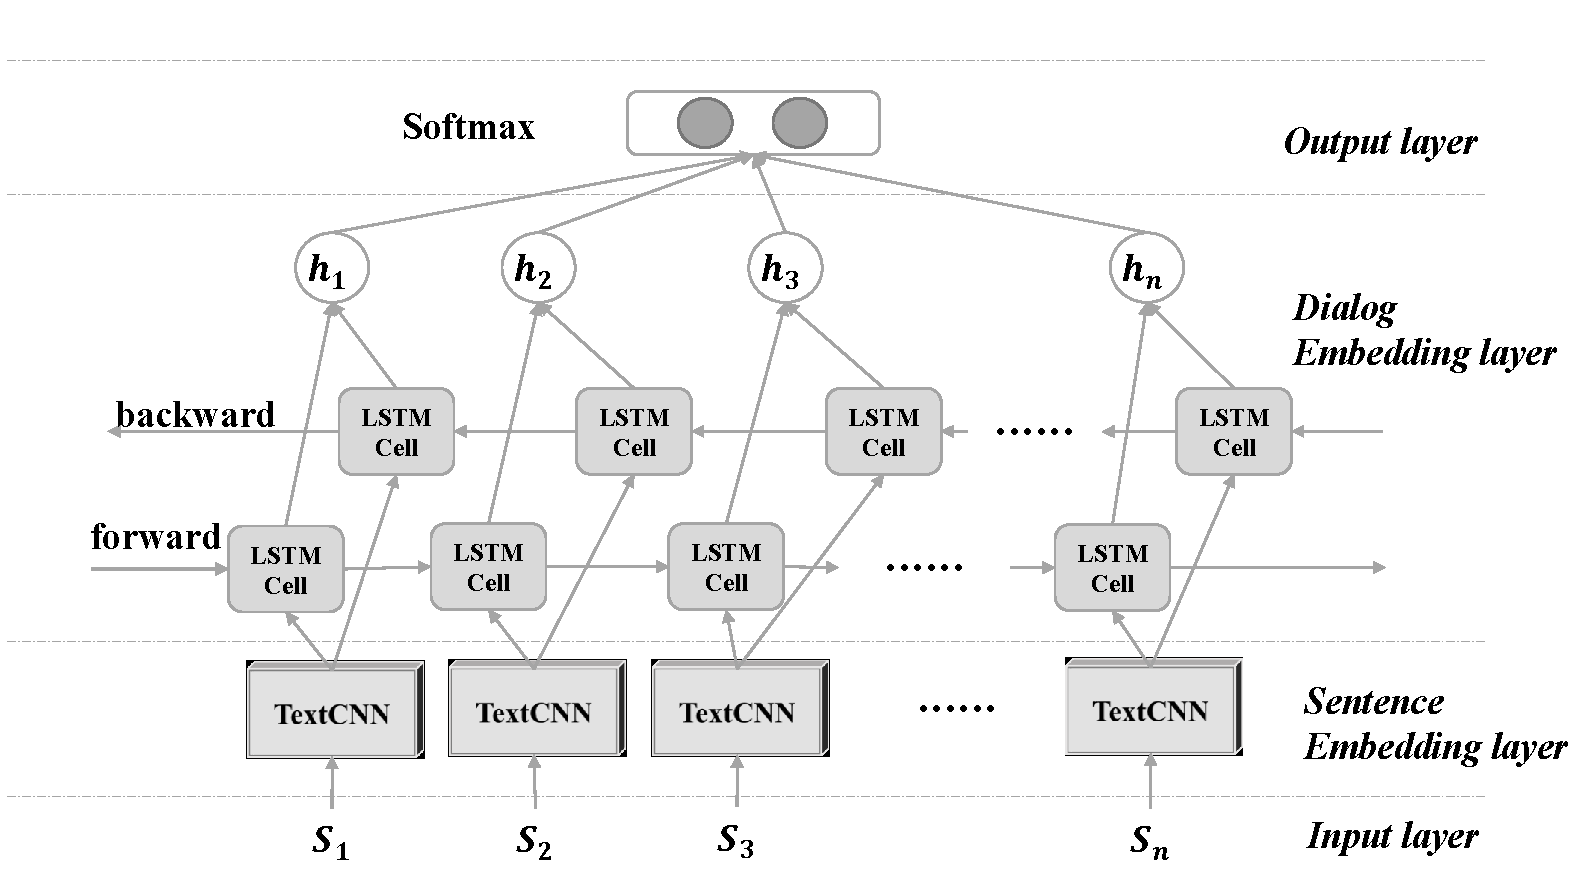
\includegraphics[width=\textwidth]{Img/model.pdf}
    \bicaption{p-{\tool}上下文敏感对话分类模型}{p-{\tool} Context-aware Dialog Classification Model}
    \label{fig:model}
\end{figure}
而{\tool}使用一对对话作为输入,其结构也可以通过修改p-{\tool}的结构得到。具体的,首先,移除p-{\tool}上层的分类层;拼接两个共享参数的相同的p-{\tool};最后,加上相似度度量层。

在实验部分,首先,我们使用相同大小的数据集来训练{\tool}和p-{\tool},并观察最后的效果增强。然后,我们把训练集分别增广到5倍、10倍、20倍和30倍来观察效果变化。因为{\tool}可以利用孪生网络天然的解决数据类别不均衡问题,然而,p-{\tool}不能,因此,我们通过随机上采样来均衡p-{\tool}的数据集。为了保证我们实验的准确性{\tool}和p-{\tool}使用相同的超参数进行训练,包括每层的维度,网络的深度以及学习率等。
\subsection{FRMiner的跨项目实验}
接下来,我们通过在三个开源项目数据集上验证了我们方法的泛化能力。我们迭代的使用其中两个项目作为训练集,剩下的一个项目作为测试集。为进行泛化能力对比,我们也在基线方法上进行跨项目实验。其中,实验中所用到的参数和实验5.1.2中保持一致。

\section{实验结果及分析}
\subsection{FRMiner进行需求识别的有效性实验结果及分析}
表格展示了每个项目三折交叉验证中不同方法达到的不同效果。
\begin{table}
\bicaption{每个项目在项目内通过不同方法取得的效果}{The performance achieved by different approaches for each project in intra-project validation}
    \label{tab:rq1}
    \centering
    \footnotesize% fontsize
    \setlength{\tabcolsep}{4pt}% column separation
    \renewcommand{\arraystretch}{1.2}%row space 
\begin{tabular}{|c|c|c|c|c|c|c|c|c|c|c|}
\hline
\multicolumn{2}{|c|}{\multirow{2}{*}{\diagbox{方法\qquad}{效果\qquad}}}   & \multicolumn{3}{c|}{AngularJS}                           & \multicolumn{3}{c|}{Bootstrap}                         & \multicolumn{3}{c|}{Chromium}                          \\ \cline{3-11} 
\multicolumn{2}{|c|}{}                           & Precision        & Recall           & F1               & Precision        & Recall           & F1               & Precision        & Recall           & F1               \\ \hline
\multirow{2}{*}{本文方法}        & FRMiner   & \textbf{90.28\%} & \textbf{89.73\%} & \textbf{90.00\%} & \textbf{86.28\%} & \textbf{88.78\%} & \textbf{87.52\%} & \textbf{89.00\%} & \textbf{87.00\%} & \textbf{88.00\%} \\ \cline{2-11} 
                                     & p-FRMiner & 31.71\%          & 54.17\%          & 40.00\%          & 50.00\%          & 47.80\%          & 48.98\%          & 14.00\%          & 44.00\%          & 20.00\%          \\ \hline
\multirow{2}{*}{已有研究方法}    & CNC       & 7.70\%           & 44.44\%          & 13.13\%          & 16.38\%          & 34.21\%          & 22.13\%          & 9.56\%           & 67.00\%          & 16.73\%          \\ \cline{2-11} 
                                     & FRA       & 13.67\%          & 80.33\%          & 23.35\%          & 23.00\%          & 48.67\%          & 31.00\%          & 12.00\%          & {81.00\%} & 20.00\%          \\ \hline
\multirow{4}{*}{文本分类方法} & NB        & 20.00\%          & 27.67\%          & 22.33\%          & 25.67\%          & {62.00\%} & 36.00\%          & 14.33\%          & 44.33\%          & 21.00\%          \\ \cline{2-11} 
                                     & GBDT      & 36.00\%          & 22.33\%          & 27.33\%          & 41.67\%          & 35.67\%          & 38.33\%          & 9.33\%           & 7.33\%           & 8.00\%           \\ \cline{2-11} 
                                     & RF        & 52.67\%          & 11.00\%          & 16.33\%          & 57.00\%          & 29.00\%          & 38.33\%          & 0.00\%           & 0.00\%           & NA               \\ \cline{2-11} 
                                     & FT        & 23.33\%          & 5.33\%           & 8.67\%           & 57.67\%          & 29.00\%          & 38.33\%          & 38.00\%          & 9.10\%           & 15.00\%          \\ \hline
\end{tabular}
\end{table}

其中,对于Precision、Recall、F1值最优的效果使用黑体标出。我们可以看到{\tool}在三个项目中均取得了最好的效果,平均精确度、召回率、F1值分别是88.52\%, 88.50\%, and 88.51\%。另外,p-{\tool}比所有的基线方法效果要好。表明了通过BiLSTM记忆上下文信息可以帮助从聊天记录中的文本分类任务。

对于两个句子级别的分类方法,CNN仅能取得17.33\%的平均F1值,主要是因为CNC是在问题评论语料库上训练得到的,而不是特征请求对话。然而,其依然能取得48.55\%的平均召回率,这表明在这两个领域里面应该存在着共有的分类模式。同时,基于规则的分类器FRA可以在六个基线方法中取得最高的平均召回率,其为70.00\%,并且在AngularJS和Chromium两个项目上分别可以取得80.33\%和81.00\%的召回率。虽然其精确度较低,但是FRA的预测结果包含大量真实的特征请求对话,这意味着对话信息中的特征请求句子也服从FRA的规则。另一方面,由于FRA使用基于规则的分类方法,而不是有监督的机器学习方法,FRA在挖掘大规模的聊天信息方面更加高效,并且,基于FRA较高的召回率这一优势,我们可以通过其解决标注数据初期的粗粒度召回问题。

对于四个文本分类方法,NB在其中取得了最好的效果。虽然RF取得了在四个方法里面取得最高的F1值-27.33\%,但其在Chromium项目上存在着欠拟合问题,即不能很好的建模训练数据,其原因主要在于Chromium项目数据集不充分,不能得到很好的训练并学习到相关模式。以下是本文提出的{\tool}在效果上大大超过四个传统文本分类模型的原因:
\begin{enumerate}
    \item 和传统的文本分类模型相比,神经网络模型具有更大的信息容量,尤其在建模复杂的对话模型上能取得较好的效果。
    \item 直觉上,模型分类两个对话的类别是否相似要比将每个对话分类为其类别更加容易进行学习。
    \item 由于数据集规模较小,文本分类模型存在在欠拟合问题,而由于{\tool}是一个pair-wise方法,可以将原数据集增广为较大规模,可以保证模型在充足的数据集上进行训练。
\end{enumerate}

总的来说,{\tool}效果上明显超过两个句子级别的特征请求分类方法和四个传统文本分类方法。由于CNC和FRA两个句子级别基线方法可以直接应用于聊天记录数据并且达到较高的召回率,他们在数据标注方面可以起到粗粒度召回的作用。

\subsection{孪生网络在FRMiner中的有效性实验及分析}

图\ref{fig:p-FR}展示了分别在相同数量的Single-Instance和Pair-Instance数据集上训练的p-{\tool}和{\tool}的效果。其中蓝色的条形图代表p-{\tool}的效果,其是在两折数据上训练的结果,训练数据量如图例所示。橙色的条形图代表使用孪生网络的{\tool}的效果,图例所示为Pair-Instance的数量。我们可以看到但训练样本量相同时,{\tool}比p-{\tool}取得了明显的较高的分类效果。{\tool}对于精确度、召回率、F1值分别平均提高了46.79\%,31.13\%,42.90\%。

\begin{figure}[htb]
\centering
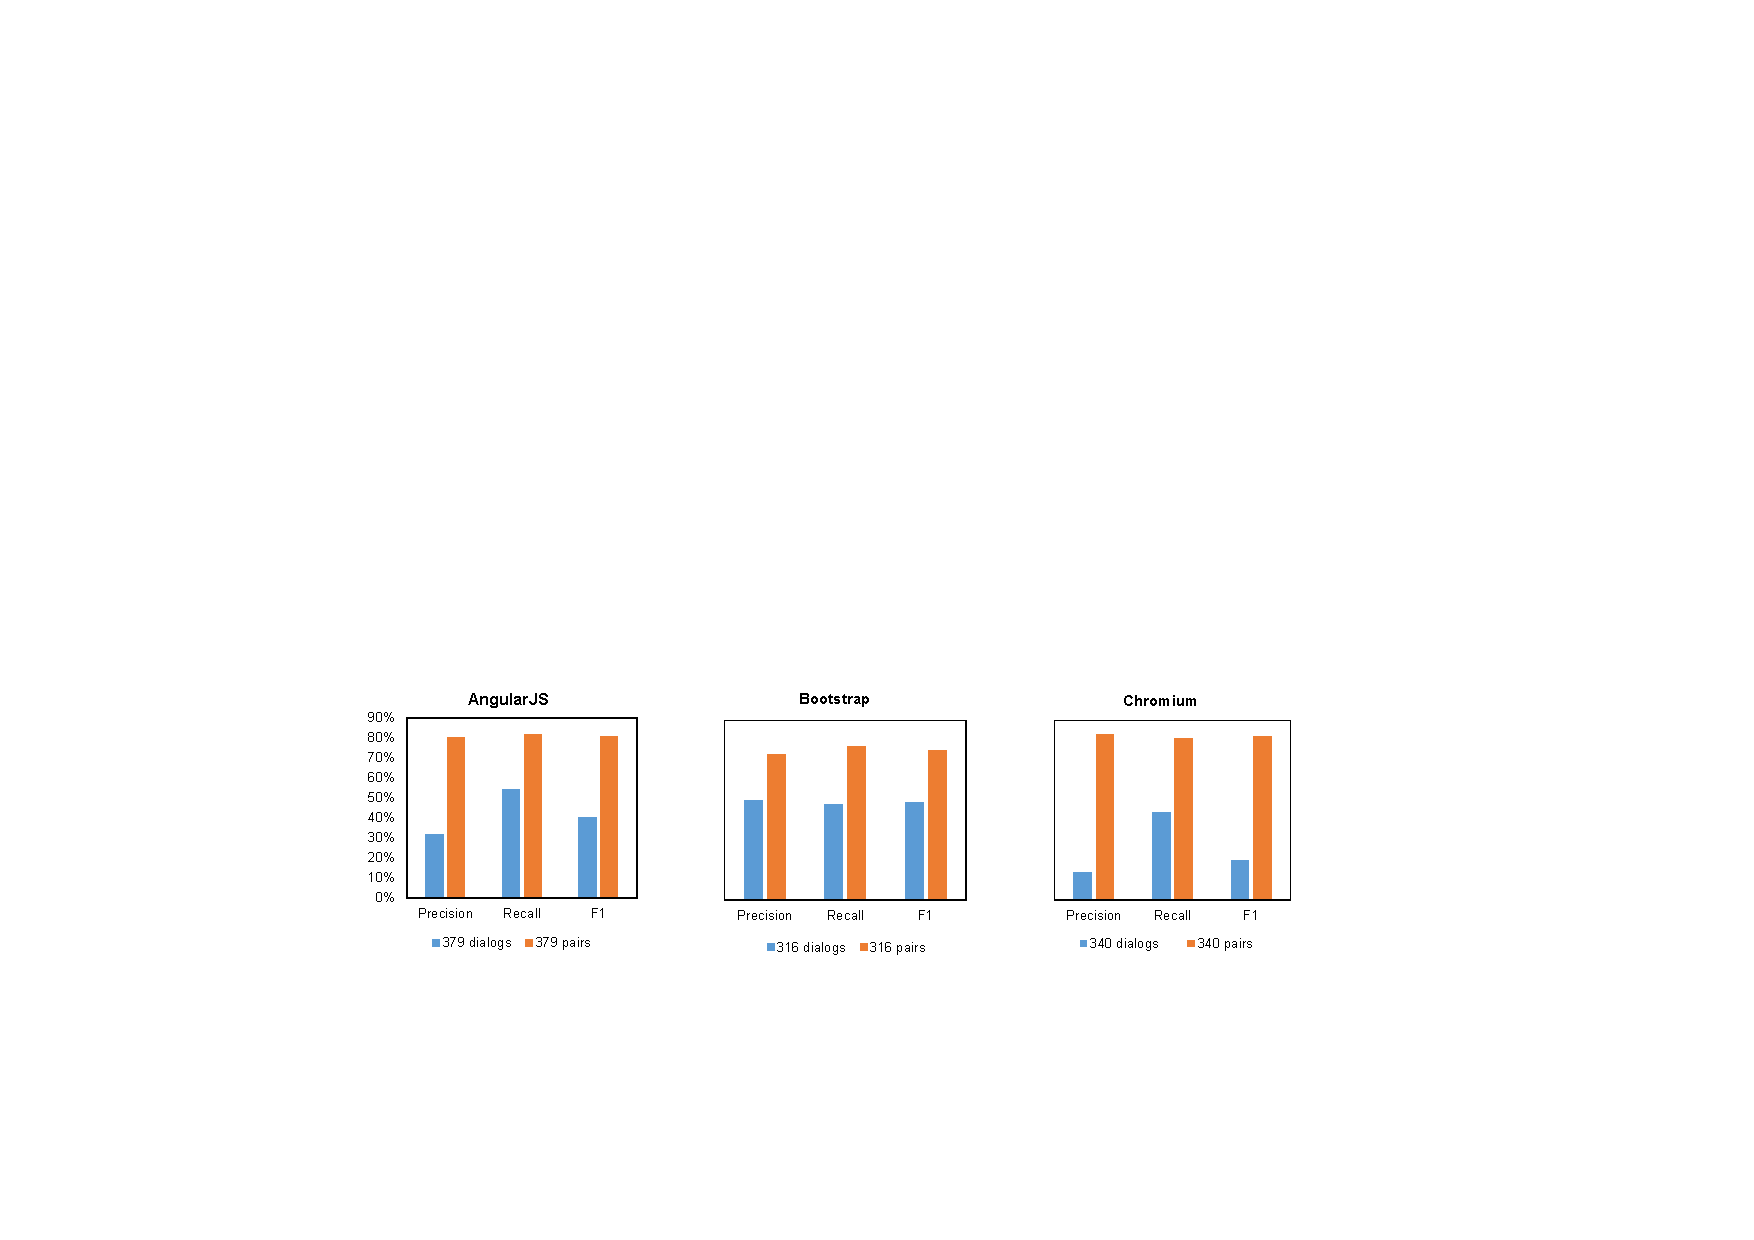
\includegraphics[width=\textwidth]{Img/p-FRvsFR.pdf}
\bicaption{p-FRMiner和FRMiner在相同大小训练集上的表现}{The comparison performances of p-FRMiner and FRMiner with the same volume of original training data}
\label{fig:p-FR}
\end{figure} 

图\ref{fig:FR-size}展示了Pair-Instance训练数据量的增广程度、分类效果的提升和在训练阶段花费的时间成本之间的关系。

\begin{figure}[htb]
\centering
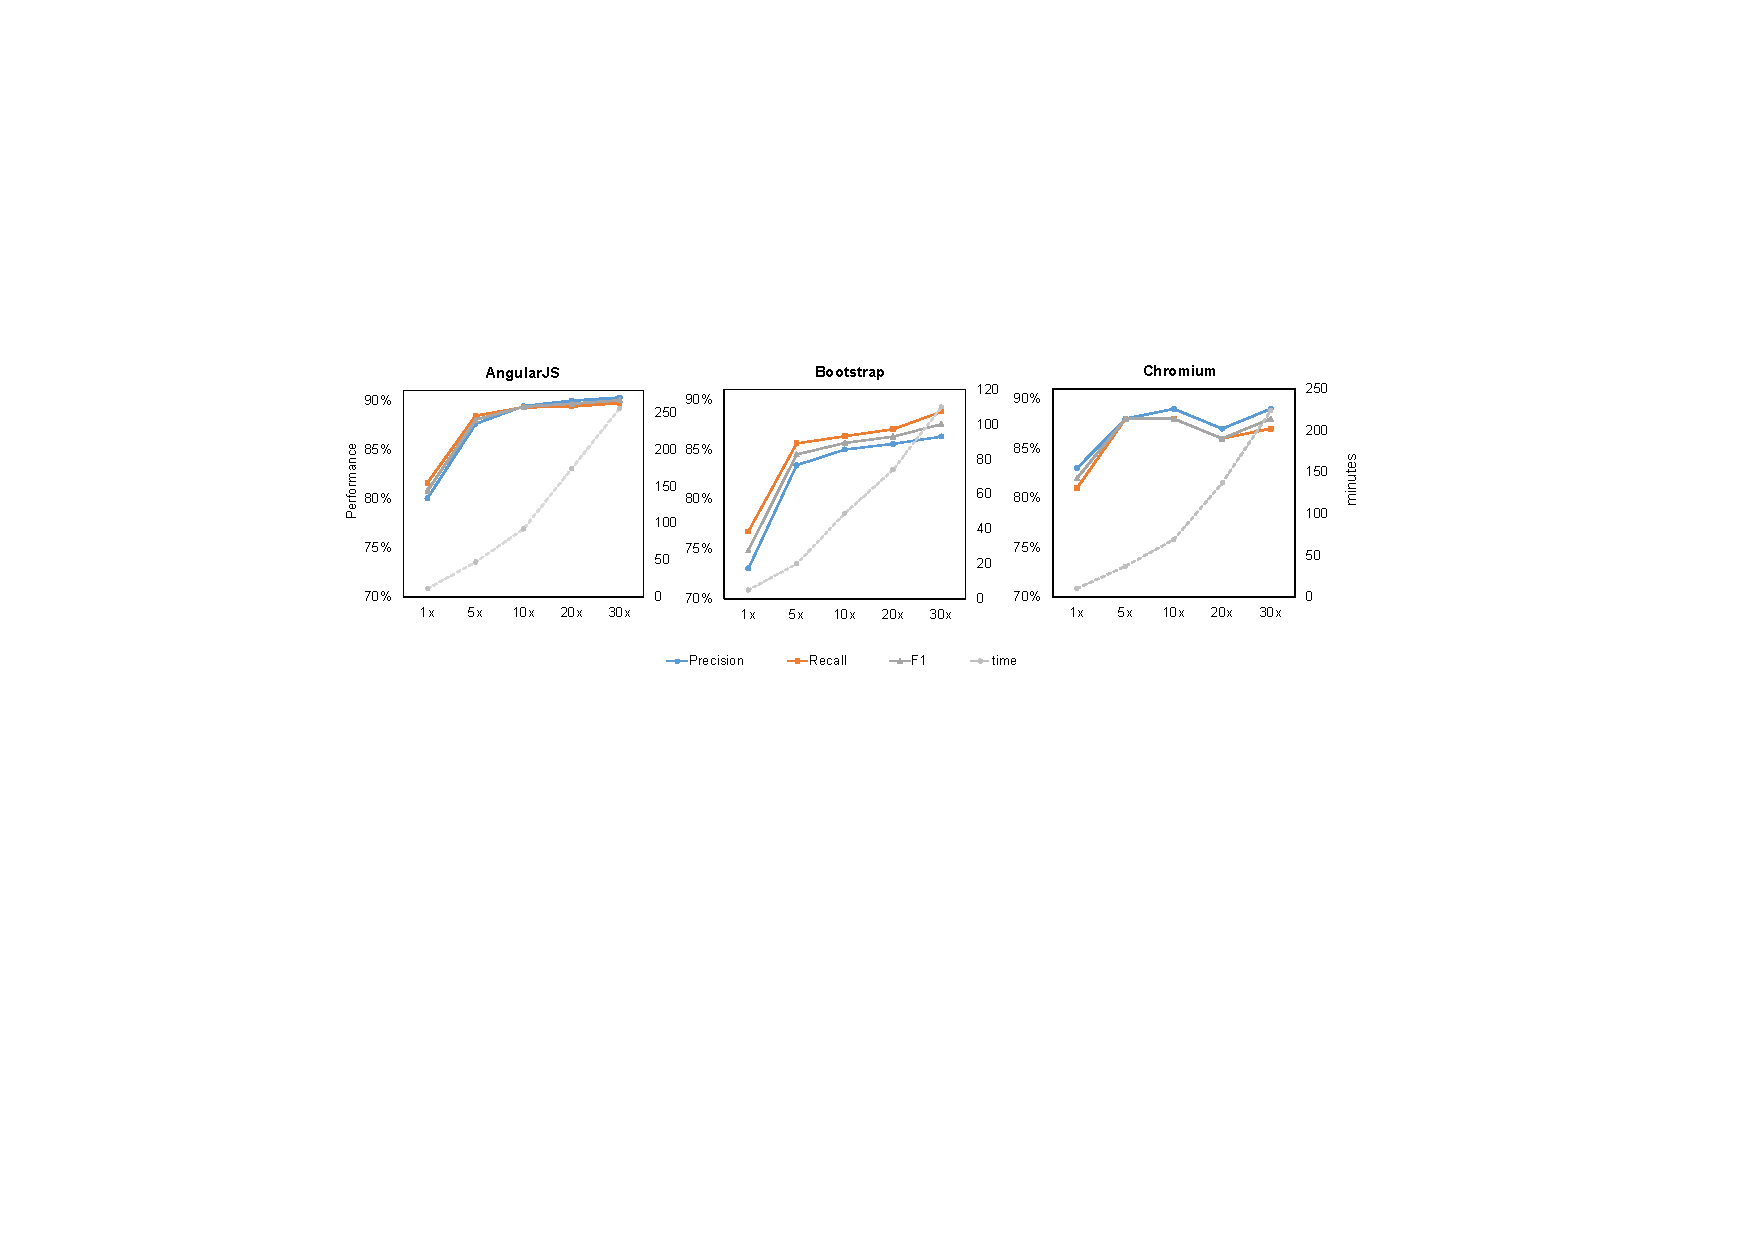
\includegraphics[width=\textwidth]{Img/FRMiner_size.pdf}
\bicaption{FRMiner在不同大小Pair数据集上的表现}{The performances of FRMiner when generating different numbers of pairs}
\label{fig:FR-size}
\end{figure} 

初始训练集数据量(1X数据量)如图\ref{fig:p-FR}所示,分别为379,316和340。我们可以看到通过扩大Pair-Instance训练集大小可以提高模型效果。当Pair-Instance训练集大小从1倍增广到30倍后,精确度、召回率、F1值分别平均提高了9.82\%,8.72\%和9\%。我们观察到模型效果在训练集扩大到5倍时提高最快,而从5倍增广到30倍时,三个项目上的效果提升较小。 当增广到20倍时,在Chromium项目上的效果甚至有较小的下降。而训练阶段所花费的时间基本呈现线性增加的特点。因此,我们认为将训练集增广到5倍是在训练效率和模型效果之间的一个较好的均衡的值。

总结来说,{\tool}比p-{\tool}可以更好地解决对话分类问题,在模型精确度、召回率、F1值上平均提升较大。实验结果表明了在训练数据较少的情况下,分辨两个对话是否同属于特征请求对话要比对单个对话分类为其类别更加简单。我们在实验中使用了5倍数据增广,因为更大的数据增强增加了模型训练时间成本,同时并不能带来更好的模型效果,而5倍数据增广较好的平衡了模型效果和训练时间成本。

\subsection{FRMiner的跨项目实验及分析}

表格\ref{tab:rq3}展示了在跨项目实验中每个项目作为测试集的表现。


\begin{table}[!htbp]
\bicaption{每个项目在跨项目实验中使用不同方法达到的效果}{The performance achieved by different approaches for each project in cross-project validation}
\label{tab:rq3}
    \centering
    \footnotesize% fontsize
    \setlength{\tabcolsep}{4pt}% column separation
    \renewcommand{\arraystretch}{1.2}%row space 
\begin{tabular}{|c|c|c|c|c|c|c|c|c|c|c|}
\hline
\multicolumn{2}{|c|}{}                                             & \multicolumn{3}{c|}{AngularJS}                                                                     & \multicolumn{3}{c|}{Bootstrap}                                                                   & \multicolumn{3}{c|}{Chromium}                                                                    \\ \cline{3-11} 
\multicolumn{2}{|c|}{\multirow{-2}{*}{\diagbox{方法\qquad}{效果\qquad}}}                    & Precision                      & Recall                         & F1                             & Precision                      & Recall                         & F1                             & Precision                      & Recall                         & F1                             \\ \hline
                                      & FRMiner                    & \textbf{85.23\%}               & \textbf{86.56\%}               & \textbf{85.89\%}               & \textbf{86.84\%}               & \textbf{85.89\%}               & \textbf{86.37\%}               & \textbf{85.87\%}               & \textbf{86.81\%}               & \textbf{86.34\%}               \\ \cline{2-11} 
\multirow{-2}{*}{本文方法}        & p-FRMiner                  & 31.03\%                        & 50.00\%                        & 38.30\%                        & 27.56\%                        & 69.08\%                        & 39.40\%                        & 16.00\%                        & 50.00\%                        & 24.24\%                        \\ \hline
                                      & {CNC} & {7.70\%}  & {44.44\%} & {13.13\%} & {16.38\%} & {34.21\%} & {22.13\%} & {9.56\%}  & {67.00\%} & {16.73\%} \\ \cline{2-11} 
\multirow{-2}{*}{已有研究方法}    & {FRA} & {13.67\%} & {80.33\%} & {23.35\%} & {23.00\%} & {48.67\%} & {31.00\%} & {12.00\%} & {81.00\%} & {20.00\%} \\ \hline
                                      & NB                         & 16.00\%                        & 75.00\%                        & 26.00\%                        & 27.00\%                        & 36.00\%                        & 31.00\%                        & 7.00\%                         & 26.00\%                        & 12.00\%                        \\ \cline{2-11} 
                                      & GBDT                       & 18.00\%                        & 14.00\%                        & 16.00\%                        & 30.00\%                        & 11.00\%                        & 16.00\%                        & 20.00\%                        & 19.00\%                        & 19.00\%                        \\ \cline{2-11} 
                                      & RF                         & 28.00\%                        & 14.00\%                        & 19.00\%                        & 37.00\%                        & 9.00\%                         & 15.00\%                        & 12.00\%                        & 26.00\%                        & 16.00\%                        \\ \cline{2-11} 
\multirow{-4}{*}{文本分类方法} & FT                         & 32.00\%                        & 19.00\%                        & 24.00\%                        & 43.00\%                        & 13.00\%                        & 20.00\%                        & 19.00\%                        & 11.00\%                        & 14.00\%                        \\ \hline
\end{tabular}
\end{table}

其中,最优的精确度、召回率、F1值使用黑体表示。需要注意的是,因为CNC和FRA是基于各自数据集训练的模型或者提取的规则,其不适用于跨项目实验,因此CNC和FRA的效果和5.1.1中项目内三折交叉实验的结果相同,为了对比和分析,我们将表格\ref{tab:rq1}中的数据复制到表格\ref{tab:rq3}中。我们可以看到{\tool}在跨项目实验中表现较好。平均F1值仅相比5.1.1中项目内实验降低2.27\%。其主要原因在于不同项目中表达特征请求的对话存在着共有的模式,并且可以在项目间进行共享。实验结果表明{\tool}可以学习到特征请求相关的范式,并且可以泛化到其他项目中,这表明开发者在不同的社区和项目中使用相似的模式表达特征请求。对于p-{\tool},其平均F1值相比项目内实验降低了10.51\%。

对于四个文本分类基线方法,NB取得了最高的F1值-23\%,并且相比项目内实验仅降低了3.44\%。我们注意到大多文本分类方法的模型效果在Angular和Chromium两个项目上比项目内实验要高,其主要是由于以下原因:
\begin{enumerate}
    \item 交叉项目实验中的训练数据集包含两个项目的数据集,而项目内实验仅包含一个项目的2/3大小的数据集。交叉项目实验可以在更充分的训练数据上进行训练。
    \item 由于交叉项目实验包含两个项目的数据集,更广泛领域的数据集可以通过引入不同领域的偏置信息帮助分类器增加泛化能力。
\end{enumerate}

因此,{\tool}在未训练数据集上依然能取得较好的效果,这表明{\tool}在不同项目见具有较好的泛化能力。同时,NB是在所有文本分类方法中从聊天记录中挖掘特征请求对话最好的方法。

\section{本章小结}

本章主要介绍针对我们提出的{\tool}设计了三个实验,包括{\tool}进行需求识别的有效性实验、孪生网络在{\tool}中的有效性实验以及{\tool}的跨项目实验的实验设置和参数配置。然后我们针对实验结果进行分析,试验结果表明我们的方法相较于两个句子级别的特征请求识别方法和四个文本分类方法有较大的性能提升,其中CNC和FRA召回率较高,在四个文本分类方法中NB的效果最好。另外由于开发者在不同项目之间通常使用相似的模式表达特征请求,因此对于捕获语法、语义能力较强的{\tool},其在跨项目中表现较好。
% \chapter{需求对话识别工具实现}

本章主要介绍从数据集构建到模型实现等代码工程实现,对{\tool}的工作流程结构进行阐述,并且介绍{\tool}在工业生产环境部署流程情况。


\section{数据集读取模块实现}

不同于传统的文本分类模型,我们在数据集构建阶段需要分别对训练集和测试集进行Pair-Instance数据集构建。因此,我们针对p-FRMiner和FRMiner同时实现Single-Instance和Pair-Instance的数据集构建方法。对于p-FRMiner和FRMiner,我们同时实现两种数据集读取方式:lazy读取和一次性加载内存方式。其中lazy方式每次读取一行,然后构建对应Instance,也可以每次读取并构建一个Batch的Instance,以避免数据集过大不能同时加载到内存从而导致的程序运行问题。

对于数据集构建和接下来模型实现方面,我们使用AllenNLP\footnote{https://allennlp.org/},一个基于PyTorch\footnote{https://pytorch.org/}构建的开源NLP库。其中p-{\tool}和{\tool}实现的数据集读取类均继承AllenNLP的\textit{Dataset Reader}类。
p-FRMiner实现的Dataset Reader中的Instance包含三个元素:dialog矩阵,矩阵的每一行为一个句子分词后的词序列,句子组成的行序列对应句子在原对话中的序列;pos-tag矩阵,矩阵的每一行为一个句子分词后对应的pos-tag序列,句子组成的行序列对应句子在原对话中的序列,因此,pos-tag矩阵中的每个元素对应dialog矩阵每个元素词的pos-tag;label标签,分别以\textit{feature}和\textit{other}代表\textit{feature dialog}和\textit{non-feature dialog}。

而FRMiner为了组建Pair-Instance,其Dataset Reader的实现方式与p-FRMiner的Dataset Reader有所不同。在构建训练集时,遍历原始Single-Instance数据集,对于一个Dialog Instance—— $Dialog_1$,我们从训练集中同时采样一个正样本,也即label为\textit{feature}的$Dialog\_pos$和一个负样本$Dialog\_neg$,和$Dialog_1$组成两个Pair-Instance,即$<Dialog_1,Dialog\_pos>$和$<Dialog_1,Dialog\_neg>$,为了控制数据增强后数据集的大小以及避免增大随机采样带来的误差,我们对以上流程在整个数据集上及进行$iter\_num$次。对于Pair-Instance,其有以下元素组成:dialog1矩阵,矩阵的每一行为一个dialog中一个句子分词后的词序列,句子组成的行序列对应句子在原对话中的序列;pos-tag1矩阵,矩阵的每一行为一个dialog中一个句子分词后对应的pos-tag序列,句子组成的行序列对应句子在原对话中的序列,因此,pos-tag1矩阵中的每个元素对应dialog1矩阵每个元素词的pos-tag;dialog2和pos-tag2矩阵同理为另一个dialog的分词以及分词后对应的pos-tag矩阵;label标签,分别以\textit{feature}和\textit{non-feature}代表\textit{feature dialog}和\textit{non-feature dialog};label\_tags标签,其形式如\textit{feature@non-feature},代表Pair-Instance中的两个dialog原始标签分别为\textit{feature}和\textit{non-feature},保存原始标签的目的是为在训练集和测试集上进行类别推断而进行针对Single-Instance的效果评估。

在获取p-FRMiner和FRMiner对应的Instance后,我们需要讲Instance矩阵转为向量化表达从而进行训练。这里,我们使用AllenNLP的\textit{ListField}、\textit{TextField}和\textit{LabelField}类将原Tensor的字符串元素如词、pos-tag、字符串label转为对应整数型索引。然后AlleNLP在以上类里面将原始Tensor转换为以整数型索引表示的神经网络输入Tensor。

\section{对话分类模块实现}

模型构建部分我们主要继承AllenNLP的\textit{Model}方法,其实现了NLP中一些常见的方法,如Vocabulary中word到index的映射、参数初始化、正则项等。继承AllenNLP的基类方法可以为我们的原型实现减少大量的重复工作。

不同于传统的单文本目标分类任务,孪生网络使用两个相同结构、共享参数的编码器对文本进行embedding,然后使用相似度度量层对Pair-Instance进行相似性评估。我们对此并没有在代码中实现两个相同的网络,而是将两个对话分别输入到同一个上下文敏感对话模型中得到两个对话的embedding表示。

对于分层的上下文敏感对话模型实现部分按照如图\ref{fig:model}所示。考虑到NLP中批处理训练需要对不同长度文本句子进行padding,并且我们的输入不同于以[batch\_size, max\_sentence\_length]为输入的句子文本分类模型,其中max\_sentence\_length为大小为bath\_size的句子中的最长长度,对话模型的输入为[batch\_size, max\_utterance, max\_sentence\_length],其中max\_utterance为大小为batch\_size的输入对话中最大的句子数,max\_sentence\_length为所有对话中最长的句子长度,因此我们需要实现三维的padding方法,使对话输入Tensor能够进行批处理训练。不同于基本的TextCNN对句子分类的输入,我们在句子Embedding层使用不同大小卷积核的TextCNN,因此对于长度小于卷积核大小的句子,我们需要将其padding为卷积核大小长度。同样的,我们需要对pos-tag embedding 的三维Tensor进行padding,然后对word embedding和pos-tag embedding进行拼接。在对三维的输入Tensor进行padding之后,我们使用AllenNLP中的\textit{CnnEncoder}对batch中每个对话的每个句子使用TextCNN进行表示,由于对于TextCNN的输入为二维Tesnor,对此,我们将输入Tensor转换为形状为[batch\_size * max\_utterance, max\_sentence\_length]的二维形式。在经过TextCNN后,我们获取所有句子的embedding表示,然后还原为[batch\_size, max\_utterance, cnn\_out\_dimension],其中cnn\_out\_dimension为TextCNN的输出维度。在对话建模层,我们使用BiLSTM,以每个句子的embedding作为输入Term对对话句子的序列信息进行双向编码,然后,可以得到对话的最终向量化表示。

针对对话的相似度度量,我们构建双层、以Sigmod为激活函数的线性层作为黑盒网络,同时接受两个对话embedding拼接的结果作为输入,输出为对话的相似性概率。因为我们在Pair-Instance数据集构建的过程中构建了相似度标签-\textit{same}和\textit{diff},因此相似度度量网络在输入对话和对应的label下可以进行训练并更新参数,从而拟合领域特定的对话相似性度量函数。对于label为\textit{same}和\textit{diff}的Pair-Instance数据,在经过以上下文敏感模型为基模型的孪生网络和相似度度量层之后,其输出分类为\textit{same}和\textit{diff}的概率值,其为一个二分类问题,这里,我们使用cross-entropy作为损失函数对模型参数进行更新优化。


\section{训练及模型调参}
我们对于训练过程使用AllenNLP的\textit{Trainer}类,其实现了一些神经网络训练过程中常用的方法,如序列化保存、GPU训练、数据集加载、梯度裁剪、TensorBoard可视化等。训练过程中所需要的参数保存在json文件中,AllenNLP加载json文件并初始化\textit{Trainer}类,然后开始进行训练以及评估测试。

对于超参数,我们使用Grid Search\cite{Bergstra2012Random}作为参数选择方法以获得最佳效果。pos-tag向量的维度为50,与单词向量相同。然后,我们可以使用$s=[w_1,w_2\dots w_n]$ 作为句子的表示形式,其中$w_i=[we_i\oplus pos_i]$。为了获得由不同尺度的局部信息组合而成的更充分的语义信息,我们对句子应用具有不同大小的多个卷积核。我们设置了4种不同的卷积核大小,分别是2、3、4、5,每类卷积核有25个。BiLSTM的输出尺寸为300(每个方向150)。我们使用线性层作为相似性度量层,然后将300维向量映射到两个值,这些值表示两个类别的概率得分。由于该任务可以视为分类问题,因此我们将交叉熵用作损失函数。

此外,为避免过拟合问题,我们以0.1的dropout rate对输入向量进行Dropout \cite{srivastava2014dropout},这意味着将随机屏蔽10%的神经元以减少每次批量训练中需要训练的参数。我们还使用了Early Stopping\cite{prechelt1998early}的策略,如果测试数据集的效果在10个Epoch内未提升,则训练过程将停止。对于神经网络的优化器,由于Adam\cite{kingma2014adam}对梯度的一阶矩估计和二阶矩估计进行综合考虑,并且其具有自适应性能好、参数的更新不受梯度的伸缩变换影响等特点,我们使用Adam优化器对模型参数进行更新优化。

\section{实际工作流应用场景部署}
我们的方法可以通过将{\tool}集成到发布团队的工作流中帮助收集群体需求。首先,发布团队需要构建聊天信息监测器或者爬虫来定期从公司的聊天平台收集对话文本信息。然后,使用自动化脚本\cite{kummerfeld2018large}来对原始对话文本进行预处理和对话解耦。接下来,通过前面介绍的对话表示和对话分类过程,{\tool}可以记录所有在表达特征请求的对话。而发布团队可以使用RSS(Really Simple Syndication)订阅定期监测收集到的隐含的特征请求对话结果。另外,由于开发者倾向于使用较为一致的方式在对话中表达特征请求,如“需要在下个版本中实现某功能”、“某功能将会一种解决方法/改进”等,因此仅当数据集的质量或聊天内容发生较大的偏移时{\tool}需要进行重新训练,否则{\tool}不需要经常进行重新训练。

% 另外,考虑到开发环境中尤其是开源社区会存在多种语言的对话如英文等,我们的方法也能很好的集成到其他语言环境中。 In addition, {\tool} can be applied to the other languages since our deep contextual dialog model has a strong ability in capturing semantic patterns. When switching to other languages, {\tool} users need to adapt the pre-trained word embedding model to the specific language. They also need to consider to apply extra preprocessing according to the specific language, e.g., apply word segmentation to Chinese corpus. Another limitation of {\tool} on language switching is related to the pre-trained dialogues disentanglement model. A new dataset needs to be annotated for retraining the model, which may involve a relatively high cost.


\section{本章小结}

本章设计并实现了我们提出的{\tool},并针对数据集构建过程进行介绍。首先我们介绍Pair-Instance数据集构建,接下来从工程实现角度介绍分层上下文敏感对话模型构建、孪生网络对话分类模型构建以及训练阶段和调参阶段细节。最后我们介绍了{\tool}如何在工业实际场景进行部署。
\chapter{总结与展望}
\section{论文工作总结}
\section{未来研究工作}
%---------------------------------------------------------------------------%
% main content
%-
%-> Appendix
%-
\cleardoublepage%
\appendix% initialize the environment
\input{Tex/Appendix}% appendix content
%-
%-> Backmatter: bibliography, glossary, index
%-
\backmatter% initialize the environment
\intotoc*{\cleardoublepage}{\bibname}% add link to toc
\bibliography{Biblio/ref}% bibliography
%---------------------------------------------------------------------------%
%->> Backmatter
%---------------------------------------------------------------------------%

\chapter[致谢]{致\quad 谢}\chaptermark{致\quad 谢}% syntax: \chapter[目录]{标题}\chaptermark{页眉}
\thispagestyle{noheaderstyle}% 如果需要移除当前页的页眉
%\pagestyle{noheaderstyle}% 如果需要移除整章的页眉

在中科院软件所互联网实验室攻读硕士研究生的三年即将结束,这段时间里,我不仅锻炼了自己的科研能力,更学会了团队的合作能力,这一切都要感谢各位老师和同学的帮助。

首先需要感谢的是我的导师王青研究员。王老师无论是从科学研究,工程实践
还是生活上都给予了我很大的帮助。王老师治学严谨、在科研领域具有丰富的经验并且待
人温和。通过和王老师的讨论交流,我不仅学习到了严谨的科研方法,还感受到一个优秀的科研工作者和教师所具备的责任感和奉献精神。在此祝愿王老师身体健康、阖家幸福。

感谢石琳老师在我科研实验以及论文写作中的悉心指导,为论文工作提出很多有价值的改进意见,强化了我的科研习惯以及论文写作能力,帮助我顺利的完成硕士期间的工程实践和科研工作。同时也要感谢王俊杰老师和王丹丹老师,她们在我的研究生期间提出了很多宝贵的建议,并在我的学习工作上给予了很大的帮助。

感谢李明阳师兄、王亚文师兄和陈磊师兄在研究生期间对于工程项目和科研工作上对我的帮助,在工程项目中,我们通力合作,一起解决了项目中遇到的各种困难,在这期间大大提高了我的工程能力和团队合作能力;在科研工作中,感谢师兄们给予的宝贵经验,帮助我更好的完成科研工作。感谢胡渊喆师兄、李守斌师兄在工作、生活中给予的帮助。感谢互联网实验室所有的师兄师姐在这三年以来对我的帮助,让我在这三年里面学习到很多。在此希望实验室发展越来越好,产出更多的科研成果。

感谢皇甫幼峰同学硕士期间一起工作、学习和讨论交流,感谢舍友吴杉同学、谭浩同学和王新刚同学三年间的鼓励和陪伴。

感谢家人和朋友的爱护和支持,使我顺利度过硕士期间生活和科研中遇到的困难和挫折。

最后感谢参与论文评审和答辩工作的各位老师以及答辩秘书,你们辛苦了。


\chapter{作者简历及攻读学位期间发表的学术论文与研究成果}

% \textbf{本科生无需此部分}。

\section*{作者简历}

2013年9月——2017年6月,在华中科技大学软件学院获得学士学位。

2017年9月——2020年7月,在中国科学院大学软件研究所攻读硕士学位。

\section*{已发表(或正式接受)的学术论文:}

{
\setlist[enumerate]{}% restore default behavior
\begin{enumerate}[nosep]
    \item Lin Shi*, \textbf{Mingzhe Xing*}, Mingyang Li, Yawen Wang, Shoubin Li, Qing Wang. Detection of Hidden Feature Requests from Massive Chat Messages via Deep Siamese Network . In 42nd International Conference on Software Engineering (ICSE’20), October 5-11, 2020, Seoul, Republic of Korea.
\end{enumerate}
}

\section*{投稿中(或在评审中)的学术论文:}

{
\setlist[enumerate]{}% restore default behavior
\begin{enumerate}[nosep]
    \item Lin Shi, Mingyang Li, \textbf{Mingzhe Xing}, Yawen Wang, Qing Wang, Xinhua Peng, Weimin Liao, Guizhen Pi, Peisheng Li. HyFinder: A Hybrid Function Extractor for Automated Requirement Analysis.投稿至FSE2020(International Symposium on Foundations of Software Engineering)
    \item Mingyang Li, Yawen Wang, \textbf{Mingzhe Xing}, Lin Shi, Qing Wang. Semi-Supervised Character-level Data Function Point Recognition with Low Labeled Resource.投稿至ICSME2020(International Conference on Software Maintenance and Evolution)
\end{enumerate}
}


\section*{参加的研究项目及获奖情况:}

{
\setlist[enumerate]{}% restore default behavior
\begin{enumerate}[nosep]
    \item 国家自然科学基金青年项目:“面向社交媒体的需求智能发现和分析方法”(项目编号:61802374),2019.1-2021.12
    \item 国家自然科学基金重点项目:“软件生命期数据组织、分析及应用研究”(项目编号:61432001),2015.1-2019.12
    % \item 国家科学基金项目:“众测环境下测试报告的智能筛选方法研究”(项目编号:61602450),2017.1-2019.12
    \item 国家重点研发计划项目:信息产品及科技服务集成化众测服务平台研发与应用(项目编号:2018YFB1403400),2019.7-2022.6
    \item “**银行智能软件研发效能研究项目”,2018.8-2020.8
\end{enumerate}
}

\cleardoublepage[plain]% 让文档总是结束于偶数页,可根据需要设定页眉页脚样式,如 [noheaderstyle]
%---------------------------------------------------------------------------%
% other information
\end{document}
%---------------------------------------------------------------------------%

